%%%%%%%%%%%%%%%%%%%%%%%%%%%%%%%%%%%%%%%%%%%%%%%%%%%%%
%% File: main.tex
%% Author: Evangelos Stamos (estamos@e-ce.uth.gr)
%% Last update: January, 2020
%% Description: Provides an example of a Diploma Thesis 
%% using the ntua-thesis pdfLaTeX class.
%%
%% Character encoding: UTF-8
%%%%%%%%%%%%%%%%%%%%%%%%%%%%%%%%%%%%%%%%%%%%%%%%%%%%%
%
%
%%%%%%
% 1. use the "modern" or "classic" option to switch between 
% a modern or classic font, respectively.
%
% 2. add/remove the "hyperref" option to enable/disable hyperlinks:
% (remember to remove auxiliary files after adding/removing 
% the "hyperref" option).
%
% 3. add/remove the "printer" option to typeset a printer-friendly 
% (grayscale)/color version of the thesis.
%
% 4. use the "watermark" option to indicate that this is not an actual
% thesis.
%
% 5. use the "histinit" option to enable "historiated initials".
% (If used, all chapter initials declared by the \InitialCharacter{}
% macro are enlarged. If omitted, arguments of \InitialCharacter{}
% are typeset as normal text.)
%
% 6. use the "plain" option to disable tikz graphics in title page
% and part/chapter headers (might help to avoid compilation timeouts).
% Note that "plain" disables CD label and CD cover creation.
%
% 7. use the "noindex" option to (hopefully) avoid compilation timeouts
% when compiling online (disables index generation - note that "\indexGR",
% "\indexEN" invocations need not be removed when toggling this option).
%
% 8. activate the "newlogo" option to use the new official Logo.
%
%%%%%%%%%%%%%%%%%%%%%%%%%%%%%%%%%%%%%%%%%%%%%%%%%%%%%%%%%%%%%%%%%%%%%%%%%%%%%%%
%
\documentclass[modern,hyperref,watermark,histinit,noindex,plain,newlogo]{ntua-thesis}
%
%%%%%%%%%%%%%%%%%%%%%%%%%%%%%%%%%%%%%%%%%%%%%%%%%%%%%%%%%%%%%%%%%%%%%%%%%%%%%%%
%
%
%%%%%%%%%%%%%%%%%%%%%%%%%%%%%%%%%%%%%%%%%%%%%%%%%%%%
%% THESIS INFO 
%%%%%%%%%%%%%%%%%%%%%%%%%%%%%%%%%%%%%%%%%%%%%%%%%%%%
%
% ΤΙΤΛΟΣ ΔΙΠΛΩΜΑΤΙΚΗΣ ΕΡΓΑΣΙΑΣ 
%
% Για εξαναγκασμένες αλλαγές γραμμής χρησιμοποιήστε "\\".
% Αν οι αλλαγές γραμμής πρέπει να είναι διαφορετικές στο εξώφυλλο σε σχέση 
% με το εσώφυλλο (σελ. 3), επαναλάβετε τον τίτλο του εξωφύλλου με τις 
% επιθυμητές αλλαγές γραμμής ως προαιρετικό όρισμα της εντολής \title.
%
% Παραδείγματα:
% 1. Όμοιος τίτλος σε εξώφυλλο και εσώφυλλο, με αυτόματες αλλαγές γραμμής:
%	    \title{Πρότυπο Σύστημα Ομότιμων Κόμβων Βασισμένο σε Σχήματα \en{RDF}}
% 2. Όμοιος τίτλος σε εξώφυλλο και εσώφυλλο, με αλλαγή γραμμής μετά τη λέξη
% "Σύστημα":
%	    \title{Πρότυπο Σύστημα \\ Ομότιμων Κόμβων Βασισμένο σε Σχήματα \en{RDF}}
% 3. Διαφορετικές αλλαγές γραμμής σε εξώφυλλο και εσώφυλλο. Στο εξώφυλλο 
% έχουμε αλλαγή γραμμής μετά τη λέξη "Σύστημα", ενώ στο εσώφυλλο η αλλαγή
% γραμμής ακολουθεί τη λέξη "Ομότιμων":
%	    \title[Πρότυπο Σύστημα \\ Ομότιμων Κόμβων Βασισμένο %
%           σε Σχήματα \en{RDF}]% (προαιρετικό όρισμα)
%           {Πρότυπο Σύστημα Ομότιμων \\ Κόμβων Βασισμένο σε %
%           Σχήματα \en{RDF}}% (υποχρεωτικό όρισμα)
%
	\title{Επαλήθευση ορθής εκτέλεσης \en{outsourced} \en{computation} με χρήση \en{Blockchain}}
%%
%
%% -------------------------------------------------------------------
%% ΥΠΟΤΙΤΛΟΣ ΔΙΠΛΩΜΑΤΙΚΗΣ ΕΡΓΑΣΙΑΣ (προαιρετικός)
%
% Αν δεν υπάρχει υπότιτλος, τοποθετήστε τον χαρακτήρα του σχολίου "%"
% πριν από την εντολή \subtitle, ή αφήστε κενό το όρισμα της εντολής.
%
% Παράδειγμα:
%%	\subtitle{Μελέτη και υλοποίηση}
	\subtitle{Μελέτη και υλοποίηση}
%
%% -------------------------------------------------------------------
%% ΤΟΥ/ΤΗΣ/ΤΩΝ
%
% "του" ή "της" ή "των", ανάλογα με το φύλο/αριθμό του σπουδαστή ή 
% των σπουδαστών
% Παράδειγμα:
%	\toutis{του}
	\toutis{του}
%
%% -------------------------------------------------------------------
%% ΟΝΟΜΑΤΕΠΩΝΥΜΟ ΣΠΟΥΔΑΣΤΗ ΣΤΑ ΕΛΛΗΝΙΚΑ (ΚΕΦΑΛΑΙΑ, ΓΕΝΙΚΗ ΠΤΩΣΗ)
%
% Για περισσότερους του ενός σπουδαστές, διαχωρίστε με ",".
% Παράδειγμα:
%	\authorNameCapitalGR{ΚΩΝΣΤΑΝΤΙΝΟΥ Δ. ΔΗΜΗΤΡΙΟΥ, ΓΕΩΡΓΙΟΥ Π. ΠΑΝΑΓΑΚΗ}
	\authorNameCapitalGR{ΓΡΗΓΟΡΑΤΟΥ Δ. ΣΠΥΡΙΔΩΝΟΣ}
%
%% -------------------------------------------------------------------
%% ΟΝΟΜΑΤΕΠΩΝΥΜΟ ΣΠΟΥΔΑΣΤΗ ΣΤΗ ΛΑΤΙΝΙΚΗ ΜΟΡΦΗ (ΠΕΖΑ)
%
% Δηλώστε εδώ τυχόν ονοματεπώνυμα στη λατινική μορφή, αλλιώς αφήστε
% κενό το όρισμα.
% Για περισσότερους του ενός σπουδαστές, διαχωρίστε με ",".
% Παράδειγμα:
%	\authorNameEN{Albert Einstein, George W. Bush} 
	%\authorNameEN{Albert Einstein} 
%
%% -------------------------------------------------------------------
%% ΟΝΟΜΑΤΕΠΩΝΥΜΟ ΣΠΟΥΔΑΣΤΗ ΣΤΑ ΕΛΛΗΝΙΚΑ (ΠΕΖΑ, ΟΝΟΜΑΣΤΙΚΗ ΠΤΩΣΗ)
%
% Για περισσότερους του ενός σπουδαστές, διαχωρίστε με ",".
% Αν τα ονοματεπώνυμα όλων των σπουδαστών είναι σε λατινική μορφή,
% αφήστε κενό το όρισμα.
% Παράδειγμα:
%	\authorNameGR{Κωνσταντίνος Δημητρίου, Γεώργιος Παναγάκης}
	\authorNameGR{Σπυρίδων Γρηγοράτος}
%
%% -------------------------------------------------------------------
%% ΟΝΟΜΑΤΕΠΩΝΥΜΟ ΕΠΙΒΛΕΠΟΝΤΑ ΚΑΘΗΓΗΤΗ
% 
	\supervisor{Νεκτάριος Κοζύρης}
%
%% -------------------------------------------------------------------
%% ΤΙΤΛΟΣ ΕΠΙΒΛΕΠΟΝΤΑ ΚΑΘΗΓΗΤΗ
%
	\supervisorTitle{Καθηγητής}
%
%% -------------------------------------------------------------------
%% ΕΠΙΒΛΕΠΩΝ/ΕΠΙΒΛΕΠΟΥΣΑ
%
% "Επιβλέπων" ή "Επιβλέπουσα", ανάλογα με το φύλο του 
% Επιβλέποντα Καθηγητή
	\supervisorMaleFemale{Επιβλέπων}
%
%% -------------------------------------------------------------------
%% ΤΟΠΟΣ/ΜΗΝΑΣ/ΕΤΟΣ ΕΚΔΟΣΗΣ
%
% //TODO: Add date
	\thesisPlaceDate{Αθήνα, Οκτώβριος 2023}
%
%% -------------------------------------------------------------------
%% ΤΟΠΟΣ/ΜΗΝΑΣ/ΕΤΟΣ ΣΥΓΓΡΑΦΗΣ (Εμφανίζεται στη σελίδα των ευχαριστιών,
%% αν υπάρχει).
%
% //TODO: Add date
	\ackPlaceDate{Αθήνα, Οκτώβριος 2023}
%
%% -------------------------------------------------------------------
%% ΗΜΕΡΟΜΗΝΙΑ ΕΞΕΤΑΣΗΣ
%
% //TODO: Add date
	\examinationDate{32α Οκτωβρίου 2023}
%% -------------------------------------------------------------------
%% ΗΜΕΡΟΜΗΝΙΑ ΔΗΛΩΣΗΣ ΠΕΡΙ ΜΗ ΛΟΓΟΚΛΟΠΗΣ
%
% //TODO: Add date
	\declarationDate{32 Οκτωβρίου 2023}
%
%% -------------------------------------------------------------------
%% ΕΤΟΣ COPYRIGHT
%
	\copyrightYear{2023}
%
%% -------------------------------------------------------------------
%% ΟΝΟΜΑΤΕΠΩΝΥΜΟ 1ου ΕΞΕΤΑΣΤΗ
%
	\firstExaminer{Γεώργιος Γκούμας}
%
%% -------------------------------------------------------------------
%% ΤΙΤΛΟΣ 1ου ΕΞΕΤΑΣΤΗ
%
	\firstExaminerTitle{Αναπληρωτής Καθηγητής}
%
%% -------------------------------------------------------------------
%% ΟΝΟΜΑΤΕΠΩΝΥΜΟ 2ου ΕΞΕΤΑΣΤΗ
%
	\secondExaminer{Τσουμάκος Δημήτριος}
%
%% -------------------------------------------------------------------
%% ΤΙΤΛΟΣ 2ου ΕΞΕΤΑΣΤΗ
%
	\secondExaminerTitle{Αναπληρωτής Καθηγητής}
%%
%%
%%%%%%%%%%%%%%%%%%%%%%%%%%%%%%%%%%%%%%%%%%%%%%%%%%%%%%%%%%%%%%%%%%%%%%
%% THESIS COLORS: 
%%%%%%%%%%%%%%%%%%%%%%%%%%%%%%%%%%%%%%%%%%%%%%%%%%%%%%%%%%%%%%%%%%%%%%
%%
%% Χρώμα εξωφύλλου - κεφαλαίων
	\chaptercolor{gray!50!brown}
%%
%% Χρώμα παραρτημάτων
	\appendixcolor{brown!60!orange}
%%
%% Χρώμα υπερσυνδέσμων (αν έχει ενεργοποιηθεί η επιλογή "hyperref")
    \hyperlinkcolor{blue}
%%
%% Χρώμα τίτλου εργασίας στο εξώφυλλο (αν δεν έχει ενεργοποιηθεί 
%% η επιλογή "plain")
    \titlecolor{white}
%%
%% Χρώμα υποβάθρου (φόντου) τίτλου εργασίας στο εξώφυλλο (αν δεν έχει 
%% ενεργοποιηθεί η επιλογή "plain")
    \titlebackgroundcolor{gray!60!brown}  
%%
%%
%%%%%%%%%%%%%%%%%%%%%%%%%%%%%%%%%%%%%%%%%%%%%%%%%%%%%%%%%%%%%%%%%%%%%%
%% COVER PAGE IMAGE: 
%%%%%%%%%%%%%%%%%%%%%%%%%%%%%%%%%%%%%%%%%%%%%%%%%%%%%%%%%%%%%%%%%%%%%%
%%
%% Εικόνα εξωφύλλου (προαιρετική)
%% Στην περίπτωση κατά την οποία δεν είναι επιθυμητή η εισαγωγή εικόνας στο εξώφυλλο,
%% διαγράψτε την εντολή \coverpageimage, ή μετατρέψτε την σε σχόλιο (με "%")
%%
%% Σύνταξη:
%%          \coverpageimage{συντελεστής μεγέθυνσης}{όνομα αρχείου εικόνας [πλήρης διαδρομή]}
%%      ή
%%          \coverpageimage[tikz]{συντελεστής μεγέθυνσης}{εντολές TikZ}
%%          (στις εντολές μπορούν να περιλαμβάνονται και δηλώσεις \usetikzlibrary, κ.λπ.)
%%      
%% Παραδείγματα:
%%      - Χρήση εικόνας από το αρχείο "figures/rdf.png" με συντελεστή μεγέθυνσης 0.8:
%%          \coverpageimage{0.8}{figures/rdf.png}
%%      - Χρήση εικόνας TikZ με συντελεστή μεγέθυνσης 0.5:
%%          \coverpageimage[tikz]{0.5}{
%%              \draw[thick, gray] \foreach \x in {18,90,...,306} {
%%                  (\x:4) node{} -- (\x+72:4)
%%                  (\x:4) -- (\x:3) node{}
%%                  (\x:3) -- (\x+15:2) node{}
%%                  (\x:3) -- (\x-15:2) node{}
%%                  (\x+15:2) -- (\x+144-15:2)
%%                  (\x-15:2) -- (\x+144+15:2)
%%              };
%%          }
%%
% //TODO: Add image
%     \coverpageimage{0.8}{figures/rdf.png}
%%
%%%%%%%%%%%%%%%%%%%%%%%%%%%%%%%%%%%%%%%%%%%%%%%%%%%%%%%%%%%%%%%%%%%%%%
%
% add custom hyphenation rules here
\hyphenation{ο-ποί-α} 
%
%%%%
%
%
%%%%
\begin{document}

\maketitle

\beginfrontmatter
	
% Περίληψη
	%//TODO: Add abstract
\begin{abstract}
Ένα σύστημα ομότιμων κόμβων αποτελείται από ένα σύνολο αυτόνομων
υπολογιστικών κόμβων στο Διαδίκτυο, οι οποίοι συνεργάζονται με
σκοπό την ανταλλαγή δεδομένων. Στα συστήματα ομότιμων κόμβων που
χρησιμοποιούνται ευρέως σήμερα, η αναζήτηση πληροφορίας γίνεται με
χρήση λέξεων κλειδιών. Η ανάγκη για πιο εκφραστικές λειτουργίες,
σε συνδυασμό με την ανάπτυξη του Σημασιολογικού Ιστού, οδήγησε στα
συστήματα ομότιμων κόμβων βασισμένα σε σχήματα. Στα συστήματα αυτά
κάθε κόμβος χρησιμοποιεί ένα σχήμα με βάση το οποίο οργανώνει τα
τοπικά διαθέσιμα δεδομένα. Για να είναι δυνατή η αναζήτηση
δεδομένων στα συστήματα αυτά υπάρχουν δύο τρόποι. Ο πρώτος είναι
όλοι οι κόμβοι να χρησιμοποιούν το ίδιο σχήμα κάτι το οποίο δεν
είναι ευέλικτο. Ο δεύτερος τρόπος δίνει την αυτονομία σε κάθε
κόμβο να επιλέγει όποιο σχήμα θέλει και απαιτεί την ύπαρξη κανόνων
αντιστοίχισης μεταξύ των σχημάτων για να μπορούν να αποτιμώνται οι
ερωτήσεις. Αυτός ο τρόπος προσφέρει ευελιξία όμως δεν υποστηρίζει
την αυτόματη δημιουργία και τη δυναμική ανανέωση των κανόνων, που
είναι απαραίτητες για ένα σύστημα ομότιμων κόμβων.

Στόχος της διπλωματικής εργασίας είναι η ανάπτυξη ενός συστήματος
ομότιμων κόμβων βασισμένο σε σχήματα το οποίο (α) θα επιτρέπει μια
σχετική ευελιξία στην χρήση των σχημάτων και (β) θα δίνει την
δυνατότητα μετασχηματισμού ερωτήσεων χωρίς την ανάγκη διατύπωσης
κανόνων αντιστοίχισης μεταξύ σχημάτων, xρησιμοποιώντας κόμβους με
σχήματα \tl{RDF} που αποτελούν υποσύνολα-όψεις ενός βασικού
σχήματος (καθολικό σχήμα).

   \begin{keywords}
   Σύστημα ομότιμων κόμβων, Σύστημα ομότιμων κόμβων βασισμένο σε
   σχήματα, Σημασιολογικός Ιστός, \tl{RDF/S}, \tl{RQL}, \tl{Jxta}
   \end{keywords}
\end{abstract}



\begin{abstracteng}
\tl{A peer-to-peer system is a set of autonomous computing nodes
(the peers) which cooperate in order to exchange data. The peers
in the peer-to-peer systems that are widely used today, rely on
simple keyword selection in order to search for data. The need for
richer facilities in exchanging data, as well as, the evolution of
the Semantic Web, led to the evolution of the schema-based
peer-to-peer systems. In those systems every node uses a schema to
organize the local data. So there are two ways in order for data
search to be feasible. The first but not so flexible way implies
that every node uses the same schema. The second way gives every
node the flexibility to choose a schema according with its needs,
but on the same time requires the existence of mapping rules in
order for queries to be replied. This way though, doesn't offer
automatic creation and dynamic renewal of the mapping rules which
would be essential for peer-to-peer systems.}

\tl{This diploma thesis aims to the development of a schema-based
peer-to-peer system that allows a certain flexibility for schema
selection and on the same time enables query transformation
without the use of mapping rules. The peers use RDF schemas that
are subsets (views) of a big common schema called global schema.}

   \begin{keywordseng}
    \tl{Peer-to-peer, Schema-based peer-to-peer, Semantic Web, RDF/S, RQL, Jxta}
   \end{keywordseng}

\end{abstracteng}
% Αφιέρωση
	\thesisDedication{στους γονείς μου}
% Ευχαριστίες
	%%%%%%%%%%%%%%%%%%%%%%%%%%%%%%%%%%%%%%%%%%%%%%%%%%%%%%%%%%%%%%%%%
%%
%% use the starred version of the "acknowledgements" environment
%% to omit signatures from this section, e.g.:
%% \begin{acknowledgements*} ... \end{acknowledgements*}
%% 
%%%%%%%%%%%%%%%%%%%%%%%%%%%%%%%%%%%%%%%%%%%%%%%%%%%%%%%%%%%%%%%%%
\begin{acknowledgements}
Θα ήθελα καταρχήν να ευχαριστήσω τον καθηγητή κ. Νεκτάριο Κοζύρη
για την επίβλεψη αυτής της διπλωματικής εργασίας και για την
ευκαιρία που μου έδωσε να την εκπονήσω στο εργαστήριο Υπολογιστικών Συστημάτων. Επίσης ευχαριστώ ιδιαίτερα την Δρ.
Κατερίνα Δόκα για την καθοδήγησή της και την εξαιρετική
συνεργασία που είχαμε. Τέλος θα ήθελα να ευχαριστήσω τους γονείς
μου για την καθοδήγηση και την ηθική συμπαράσταση που μου
προσέφεραν όλα αυτά τα χρόνια.
\end{acknowledgements}
% Πίνακας Περιεχομένων
	\tableofcontents
% Κατάλογος Σχημάτων
	\listoffigures
% Κατάλογος Εικόνων
	\listofillustrations
% Κατάλογος Πινάκων
	\listoftables
% Πρόλογος
	%\include{front_matter/preface}
	
\beginmainmatter

%%%%%%%%%%%%%%%%%%%%%%%%%%%%%%%%%%%%%%%%%%%%%%%%%%%%%
%% INCLUDE YOUR CHAPTERS/SECTIONS HERE
%%
% Εισαγωγή
	\chapter{Εισαγωγή} 
\InitialCharacter{Σ}την σύγχρονη ψηφιακή εποχή, το υπολογιστικό νέφος 
\en{(cloud computing)} έχει αναδειχθεί σε ακρογωνιαίο λίθος της υποδομής
πληροφοριακών συστημάτων, προσφέροντας κλιμακούμενους υπολογιστικούς
πόρους κατά παραγγελία. Παραδοσιακά, οι υπηρεσίες υπολογιστικού νέφους 
κυριαρχούνται από τεχνολογικούς κολοσσούς, όπως οι \en{Amazon 
(Amazon Web Services)}, \en{IBM (IBM Cloud)}, \en{Microsoft (Microsoft Azure)} και 
\en{Google (Google Cloud)}. Αυτά τα συγκεντρωτικά μοντέλα, αν 
και αποτελεσματικά, συχνά στερούνται διαφάνειας στην πολιτική τιμολόγησης, 
την κατανομή των πόρων και τις διαδικασίες λήψης των αποφάσεων. 
Επιπλέον, εισάγουν πιθανές μονοπωλιακές  συμπεριφορές στην τιμολόγηση
και την προσφορά υπηρεσιών.
 
Καθώς ο κόσμος κινείται προς ένα πιο αποκεντρωμένο πρότυπο σε διάφορους 
τομείς, από τα χρηματοοικονομικά έως την αλυσίδα εφοδιασμού, το πεδίο 
υπολογιστικού νέφους δεν αποτελεί εξαίρεση. Η υπόσχεση της αποκέντρωσής 
του προσφέρει την δυνατότητα μεγαλύτερης διαφάνειας, ενισχυμένης ασφάλειας 
και δικαιότερης κατανομής των πόρων. Εξαλείφοντας του μεσάζοντες και 
αξιοποιώντας τους εγγενείς μηχανισμούς εμπιστοσύνης της τεχνολογίας 
\en{Blockchain}, το αποκεντρωμένο υπολογιστικό νέφος μπορεί να εκδημοκρατίσει 
την πρόσβαση στην υπολογιστική ισχύ και να προωθήσει μια ανταγωνιστική 
αγορά.


\section{Αντικείμενο της διπλωματικής}
Η παρούσα εργασία παρουσιάζει μια νέα προσέγγιση για την αποκέντρωση 
των υπηρεσιών υπολογιστικού νέφους μέσω της ανάπτυξης μια αποκεντρωμένης 
εφαρμογής \en{(decentralized App – dApp)} στο \en{Ethereum Blockchain}. 
Το προτεινόμενο σύστημα επιτρέπει στους χρήστες να αναθέτουν υπολογιστικές 
εργασίες γραμμένες σε \en{Java} σε ένα αποκεντρωμένο δίκτυο παρόχων. 
Μέσω ενός μηχανισμού δημοπρασιών, οι πάροχοι των υπολογιστικών πόρων 
υποβάλλουν προσφορές για την ανάληψη εργασιών και οι πελάτες επιλέγουν 
τους παρόχους που επιθυμούν βάσει ενός συνδυασμού της προσφοράς που έχει 
κατατεθεί και του ιστορικού των επιδόσεων τους. Το σύστημα διασφαλίζει την 
ακεραιότητα της εκτέλεσης των εργασιών και προσφέρει μια ασφαλή διαδικασία 
πληρωμής μετά την επιτυχή ολοκλήρωσή τους.

Τα επόμενα κεφάλαια θα εμβαθύνουν στον σχεδιασμό, την αρχιτεκτονική και 
τις λεπτομέρειες υλοποίησης της \en{dApp}, αξιολογώντας τις δυνατότητές της 
να αναδιαμορφώσει το τοπίο του υπολογιστικού νέφους και να προσφέρει ένα 
πιο διαφανές, αξιόπιστο και αποτελεσματικό σύστημα για την ανάθεση 
υπολογιστικών εργασιών σε τρίτους.



\section{Οργάνωση του τόμου}
Η παρούσα εργασία είναι οργανωμένη σε επτά κεφάλαια. Στο κεφάλαιο 2 δίνεται το θεωρητικό υπόβαθρο του \en{cloud computing} και του \en{Blockchain}, με έμφαση στο \en{Ethereum} και τις λύσεις που προσφέρει. Στο κεφάλαιο 3 παρουσιάζεται η προεπισκόπηση, ο σχεδιασμός και αρχιτεκτονική του προτεινόμενου συστήματος. Στα κεφάλαια 4 και 5 αναλύονται οι επιμέρους μηχανισμοί των δημοπρασιών και εκτέλεσης των εργασιών αντίστοιχα, ενώ στο κεφάλαιο 6 περιγράφεται η υλοποίηση του συστήματος. Τέλος, στο κεφάλαιο 7 πραγματοποιείται η πειραματική αξιολόγηση της εφαρμογής και στο κεφάλαιο 8 παρουσιάζονται τα συμπεράσματα, η σημασία τις εργασία, καθώς και οι μελλοντικές επεκτάσεις της.
% Μέρη/Κεφάλαια
	\part{Θεωρητικό Μέρος}
	\chapter{Θεωρητικό υπόβαθρο}
\InitialCharacter{Σ}το κεφάλαιο αυτό παρουσιάζονται η εξέλιξη του 
\en{Cloud Computing}, η τεχνολογία \en{Blockchain}, καθώς και οι
αποκεντρωμένες εφαρμογές. Επίσης, γίνεται αναφορά σε προηγούμενες εργασίες 
που ασχολούνται με την ιδέα του αποκεντρωμένου υπολογιστικού νέφους.

\section{\en{Cloud Computing}}
\subsection{Εξέλιξη \en{Cloud Computing}}
Το υπολογιστικό νέφος αναφέρεται στην παροχή διαφόρων υπηρεσιών μέσω του 
διαδικτύου, συμπεριλαμβανομένων της αποθήκευσης και της υπολογιστικής ισχύος. 
Η έννοια, αν και έγινε ευρέως διαδεδομένη τα τελευταία χρόνια, έχει τις ρίζες 
της στην δεκαετία του 1960 με την έλευση του \en{utility computing}. Η ιδέα 
βασιζόταν στο εγχείρημα ότι οι υπολογιστικοί πόροι, όπως το νερό και το 
ηλεκτρικό ρεύμα, μπορούν να παρέχονται σε οικίες και επιχειρήσεις ως υπηρεσία 
κοινής ωφέλειας. Ωστόσο, μόλις την δεκαετία του 2000, με την άνοδο του 
διαδικτύου υψηλής ταχύτητας, τις σημαντικές εξελίξεις στις τεχνολογίες
της εικονικοποί-ησης \en{(virtualization)} και την αύξηση της υπολογιστικής ισχύος, 
το \en{cloud computing} άρχισε να παίρνει την σύγχρονη μορφή του.

Εταιρείες όπως η \en{Amazon}, η \en{Microsoft} και η \en{Google}, ήταν από τις 
πρώτες που αναγνώρισαν τις δυνατότητες ενοικίασης των τεράστιων υπολογιστικών 
πόρων τους. Η \en{Amazon Web Services (AWS)} ξεκίνησε το 2006, σηματοδοτώντας 
την έναρξη της σύγχρονης εποχής του νέφους. Τα επόμενα χρόνια παρατηρήθηκε 
μια έκρηξη υπηρεσιών \en{cloud computing}, οι οποίες καλύπτουν διάφορες τεχνολογικές ανάγκες, 
από την υποδομή ως υπηρεσία \en{(Infrastructure as a Service – IaaS)} έως το 
λογισμικό ως υπηρεσία \en{(Software as a Service – SaaS)}.

\subsection{Υφιστάμενα συγκεντρωτικά μοντέλα και οι περιορισμού τους}
Τα συγκεντρωτικά μοντέλα υπολογιστικού νέφους, προσφερόμενα από τεχνολογικούς 
κολοσσούς όπως το \en{AWS}, το \en{Google Cloud} και το \en{Microsoft Azure}
κυριαρχούν στην τρέχουσα αγορά. Οι υπηρεσίες αυτές παρέχουν στους χρήστες 
αξιόπιστες, κλιμακούμενες και συχνά οικονομικά αποδοτικές λύσεις. 

Ωστόσο, συνοδεύονται από εγγενείς περιορισμούς:
\begin{itemize}
\item Έλλειψη διαφάνειας: Ο τρόπος τιμολόγησης μπορεί να πολύπλοκος και οι 
χρήστες συχνά δεν έχουν σαφή εικόνα για την κατανομή των πόρων.
\item Ενιαίο σημείο αποτυχίας (\en{single point of failure}): Τα συγκεντρωτικά 
συστήματα, εκ κατασκευής, έχουν πιθανά σημεία συμφόρησης. Εάν ένας μεγάλος 
πάροχος υπηρεσιών υπολογιστικού νέφους αντιμετωπίσει διακοπή λειτουργίας, 
αυτό μπορεί να επηρεάσει εκατομμύρια χρήστες.
\item Ανησυχίες σχετικά με το απόρρητο των δεδομένων: Με τα δεδομένα 
συγκεντρωμένα σε λίγες εταιρείες, υπάρχουν βάσιμες ανησυχίες σχετικά με την 
κατάχρηση, την παρακολούθησή τους, καθώς και τις παραβιάσεις των υπάρχοντων 
συστημάτων.
\item Δυνατότητα μονοπωλιακής συμπεριφοράς: Η κυριαρχία λίγων εταιρειών στην 
αγορά μπορεί να οδηγήσει σε μείωση του ανταγωνισμού και της καινοτομίας.
\end{itemize}
%//TODO: about environment too 

%//TODO: Add more about bitcoin, blockchain, ethereum, smart contracts, dApps, layers above ethereum, etc.
\section{\en{Blockchain}}
\subsection{Εισαγωγή στην τεχνολογία \en{Blockchain}}
Το 2008, μια οντότητα - άνθρωπος ή ομάδα ανθρώπων - με το ψευδώνυμο \en{Satoshi Nakamoto} παρουσίασε το \en{Bitcoin}, ένα αποκεντρωμένο ψηφιακό νόμισμα. Πέρα από τη νομισματική του λειτουργία, το \en{Bitcoin} εισήγαγε την τεχνολογία του \en{Blockchain}. 
Το \en{Blockchain} είναι μια αλυσίδα από \en{blocks}, στα οποία αποθηκεύονται οι συναλλαγές που πραγματοποιούνται στο δίκτυο. Αποτελεί, δηλαδή, μια βάση δεδομένων συναλλαγών σε ένα δίκτυο, η οποία λειτουργεί ως αποκεντρωμένο λογιστικό βιβλίο. Προσφέρει διαφάνεια, ασφάλεια και απουσία κεντρικού ελέγχου. Στον πυρήνα του, το \en{blockchain}, χρησιμοποιώντας κρυπτογραφικές αποδείξεις και έναν αλγόριθμο συναίνεσης (\en{consensus algorithm}) είναι ανθεκτικό στην τροποποίηση των δεδομένων του, διατηρώντας με τον τρόπο αυτό την ακεραιότητά τους, και εξασφαλίζει την εμπιστοσύνη μεταξύ των συμμετεχόντων.

\subsection{\en{Ethereum}}
To \en{Ethereum}, το οποίο παρουσιάστηκε το 2013 από τον \en{Vitalik Buterin} και δημοσιεύθηκε το 2015, επέκτεινε την ιδέα του \en{blockchain} και δημιούργησε μια δημόσια πλατφόρμα κατανεμημένου υπολογισμού ανοικτού κώδικα, η οποία διαθέτει την λειτουργικότητα των έξυπνων συμβολαίων. Με τον τρόπο αυτό, παρέχει στους προγραμματιστές την \en{Ethereum Virtual Machine (EVM)}, μια αποκεντρωμένη εικονική μηχανή που είναι \en{Turing complete}, μετατρέποντας τη δημιουργία εφαρμογών στο \en{blockchain} σε πολύ απλούστερη και εύκολη διαδικασία.

\subsection{Εξυπνά συμβόλαια και Aποκεντρωμένες εφαρμογές}
Μία από τις βασικές καινοτομίες του \en{Ethereum} είναι το έξυπνο συμβόλαιο (\en{smart contract}). Τα έξυπνα συμβόλαια είναι ντετερμινιστικά αυτοεκτελούμενα συμβόλαια όπου οι όροι γράφονται απευθείας σε κώδικα και διανέμονται στο \en{blockchain}. Εκτελούν αυτόματα αξιόπιστες συναλλαγές, χωρίς την ανάγκη διαμεσολάβησης τρίτου, με τρόπο ανιχνεύσιμο και μη αναστρέψιμο. Η προσθήκη των έξυπνων συμβολαίων επεκτείνει την χρήσης της τεχνολογίας \en{blockchain} πέρα από τις χρηματοοικονομικές συναλλαγές - όπως αυτές στις οποίες απευθύνεται το \en{Bitcoin} - σε οποιονδήποτε τομέα η εμπιστοσύνη είναι απαραίτητη, όπως τα συστήματα ψηφοφορίας και οι εφαρμογές \en{Internet of Things (IoT)}.

Οι αποκεντρωμένες εφαρμογές, ή \en{dApps}, είναι ένα άμεσο προϊόν της λειτουργικότητας των έξυπνων συμβολαίων, που εκτελούνται σε ένα δίκτυο \en{blockchain} με ομότιμο τρόπο. Αυτές οι εφαρμογές δεν απαιτούν κεντρική αρχή, είναι ανοικτού κώδικα και δίνουν κίνητρα στους χρήστες μέσω κρυπτογραφικών \en{tokens}. Αξιοποιούν τα οφέλη της τεχνολογίας \en{blockchain} για να διασφαλίσουν ότι καμία μεμονωμένη οντότητα δεν έχει τον έλεγχο της εφαρμογής, προσφέροντας ένα νέο επίπεδο ασφάλειας και εμπιστοσύνης για τους χρήστες.

\subsection{\en{Ether} και \en{Gas Fees}}
Το κρυπτονόμισμα του \en{Ethereum}, το \en{Ether} (\en{ETH}), εξυπηρετεί δύο βασικούς σκοπούς: την αποζημίωση των κόμβων του δικτύου για τους υπολογισμούς που εκτελούν και τη διαπραγμάτευσή του ως ψηφιακό νόμισμα σε διάφορα ανταλλακτήρια κρυπτονομισμάτων. Στο δίκτυο του \en{Ethereum}, οι αμοιβές των συναλλαγών μετρώνται με βάση την υπολογιστική πολυπλοκότητα, τη χρήση εύρους ζώνης και τις ανάγκες αποθήκευσης, οι οποίες υπολογίζονται σε όρους \en{gas} και πληρώνονται σε \en{ETH}. Αυτό διασφαλίζει ότι κακόβουλα προγράμματα ή αναποτελεσματικός κώδικας δεν φράσσουν το δίκτυο.

Για να διευκολύνει τις συναλλαγές και τους υπολογισμούς, το \en{Ethereum} χρησιμοποιεί και μονάδες μικρότερης αξίας. Η μικρότερη μονάδα του \en{Ether} είναι γνωστή ως \en{wei}. Ένα \en{Ether} ισοδυναμεί με ένα πεντάκις εκατομμύριο \en{wei} ($1 \en{wei} = 10^{-18} \en{eth}$). H αμέσως επόμενη μονάδα που χρησιμοποιείται ονομάζεται \en{gwei} (\en{Gigawei}) και ισοδυναμεί με ένα δισεκατομμύριο \en{wei} ή 0,000000001 \en{Ether}.

Αυτές οι μικρότερες μονάδες \en{Ether} είναι ζωτικής σημασίας για την ακρίβεια στις συναλλαγές, ειδικά όταν πρόκειται για χρεώσεις \en{gas}, καθώς επιτρέπουν στους χρήστες να καθορίζουν το ακριβές ποσό που είναι διατεθειμένοι να πληρώσουν ανά μονάδα \en{gas}, χωρίς να χρειάζεται να χρησιμοποιούν εξαιρετικά μικρής αξίας δεκαδικά ψηφία. Αυτό το σύστημα όχι μόνο παρέχει μια πιο κατανοητή κλίμακα για τους χρήστες, αλλά επιτρέπει επίσης στο δίκτυο \en{Ethereum} να χειρίζεται τις συναλλαγές και τις αλληλεπιδράσεις έξυπνων συμβολαίων με ακρίβεια, εξασφαλίζοντας δικαιοσύνη για όλα τα εμπλεκόμενα μέρη.

\subsection{\en{Ethereum} 2.0}
Αρχικά, το \en{Ethereum blockchain} χρησιμοποιούσε ως αλγόριθμο συναίνεσης (\en{consensus algorithm}) το \en{Proof of Work (PoW)} που χρησιμοποιεί και το \en{Bitcoin}. Το γεγονός αυτό εισήγαγε περιορισμούς στην επεκτασιμότητα του δικτύου, την ενεργειακή αποδοτικότητά του, καθώς και υψηλές χρεώσεις στις συναλλαγές. Στις 15 Σεπτεμβρίου 2022, ολοκληρώθηκε η μετάβαση στο \en{blockchain Ethereum} 2.0, το οποίο χρησιμοποιεί για \en{consensus algorithm} το \en{Proof of Stake (PoS)}, μειώνοντας έτσι την ενεργειακή κατανάλωση κατά 99\%. 

\subsection{\en{Layer 2}}
Οι τρεις επιθυμητές ιδιότητες της τεχνολογίας \en{blockchain} είναι η αποκέντρωση, η ασφάλεια και η επεκτασιμότητα. Ωστόσο, σύμφωνα με το τρίλημμα του \en{blockchain}, μια απλή αρχιτεκτονική του μπορεί να πετύχει μόνο δύο από τις τρεις. Έτσι, προς επίτευξη μιας ασφαλούς και αποκεντρωμένης αλυσίδας, πρέπει να θυσιαστεί η επεκτασιμότητα. 
Καθώς το \en{Ethereum} επεξεργάζεται σήμερα περισσότερες από 1 εκατομμύριο συναλλαγές την ημέρα, με δυνατότητα επεξεργασίας 15 συναλλαγές το δευτερόλεπτο, η συνεχώς αυξανόμενη ζήτηση για χρήση του μπορεί να προκαλέσει υψηλές χρεώσεις στις συναλλαγές.
Στο σημείο αυτό εισάγονται τα δίκτυα επιπέδου 2 (\en{layer} 2), τα οποία, ενώ χρησιμοποιούν το δίκτυο του επιπέδου 1 (\en{mainnet Ethereum}), παρέχουν τρόπους για επεξεργασία των συναλλαγών εκτός αυτού (\en{off-chain computations}). Έτσι, αφαιρούν το βάρος επιβεβαίωσης κάθε συναλλαγής από το επίπεδο 1, επιτρέποντάς του να γίνει λιγότερο συμφορημένο και όλα να γίνονται πιο κλιμακούμενα, χωρίς να θυσιάζεται η αποκέντρωση και η ασφάλεια. 



\section{Προηγούμενες εργασίες σχετικά με το αποκεντρωμένο \en{cloud computing} και τις \en{dApps}}
Οι περιορισμοί των συγκεντρωτικών μοντέλων υπολογιστικού νέφους και οι 
δυνατότητες της τεχνολογίας \en{blockchain}, οδήγησαν ερευνητές και 
προγραμματιστές να διερευνήσουν το αποκεντρωμένο υπολογιστικό νέφος. 
Έργα όπως το \en{Golem}, το \en{iExec}, το \en{Filecoin} και το \en{SONM} 
έχουν αποτολμήσει το εγχείρημα αυτό, με στόχο την δημιουργία μιας 
αποκεντρωμένης αγοράς υπολογιστικής ισχύος και κατανεμημένου αποθηκευτικού 
χώρου.
Οι πλατφόρμες αυτές επιτρέπουν στους χρήστες να νοικιάζουν τους αδρανείς 
υπολογιστικούς ή αποθηκευτικούς πόρους τους, δημιουργώντας ένα δίκτυο 
ομότιμων κόμβων.

%//TODO: Add
[Προσθήκη σχολίων και διαφορών...]

Το \en{CloudAgora} παρουσιάζεται ως μια πλατφόρμα που στοχεύει να σπάσει 
το μονοπώλιο των παραδοσιακών παρόχων υπολογιστικού νέφους. Αξιοποιεί 
την τεχνολογία \en{blockchain} για να προσφέρει μια αποκεντρωμένη αγορά 
υπολογιστικών πόρων και αποθήκευσης, επιτρέποντας σε οποιονδήποτε δυνητικό 
πάροχο πόρων να αξιοποιεί τους αδρανείς πόρους του και να ανταγωνίζεται με 
τους υπόλοιπους με ίσους όρους. Στην περίπτωση της εκτέλεσης εργασίας με 
υπολογιστικούς πόρους, για την επαλήθευση της ορθής εκτέλεσής της, 
χρησιμοποιεί το \en{TrueBit Protocol} το οποίο αποτελεί μια σύνθετη επιλογή που προσφέρει περιορισμούς, προσθέτοντας καθυστέρηση στην εκτέλεση των εργασιών και κόστος στις συναλλαγές.

To \en{ChainFaas} στοχεύει στην αξιοποίηση της υπολογιστικής ικανότητας 
των προσωπικών υπολογιστών για κατανεμημένους υπολογισμούς, αναθέτοντας 
σε αυτούς εργασίες υπολογιστικής ισχύος. Για την επίτευξη της εμπιστοσύνης, 
χρησιμοποιείται ιδιωτικό (\en{private}) \en{blockchain}, όπου μπορούν να 
συμμετάσχουν σε αυτό μόνο χρήστες που έχουν πάρει άδεια από τον διαχειριστή του δικτύου και μπορούν να ελεγχθούν ανά πάσα στιγμή, σε αντίθεση με τα δημόσια (\en{public}) \en{blockchains} όπου μπορεί να συμμετάσχει ο καθένας χωρίς την δυνατότητα 
ελέγχου.

%//TODO: Add papers, describe better the platforms, especially cloudAgora and chainFaas
[Προσθήκη/ Βελτίωση...]
    \part{Πρακτικό Μέρος} 
	\chapter{Σχεδιασμός και αρχιτεκτονική του συστήματος}
\InitialCharacter{Σ}το κεφάλαιο αυτό περιγράφεται η αρχιτεκτονική της \en{dApp} και τα σενάρια εκτέλεσης που καλύπτει. Αρχικά, παρουσιάζεται μια επισκόπηση της λειτουργίας της εφαρμογής και των συμμετεχόντων σε αυτήν. Στην συνέχεια, αναλύονται η αρχιτεκτονική της εφαρμογής τα σενάρια εκτέλεσης που καλύπτει και οι διαδικασίες που ακολουθούνται σε κάθε ένα από αυτά. Τέλος, παρουσιάζονται τα μέτρα ασφαλείας που έχουν ληφθεί για την την διασφάλιση της αξιοπιστίας της.

\section{Επισκόπηση της προτεινόμενης \en{dApp}}

Στο πλαίσιο του αποκεντρωμένου υπολογιστικού νέφους, αναδύονται 
δύο κρίσιμες προκλήσεις: η διασφάλιση της ειλικρινούς εκτέλεσης των εργασιών 
και η προστασία του περιβάλλοντος του παρόχου. Οι παραδοσιακές μέθοδοι συχνά 
περιλαμβάνουν δυσκίνητες ή δαπανηρές διαδικασίες επαλήθευσης, οι οποίες μπορεί 
να αποτελέσουν αποτρεπτικό παράγοντα για πολλούς χρήστες. Επιπλέον η εκτέλεση 
άγνωστου κώδικα στο μηχάνημα ενός παρόχου ενέχει σημαντικούς κινδύνους ασφαλείας.

Αντιμετωπίζοντας αυτές τις προκλήσεις, η \en{dApp} εισάγει δύο απλές λύσεις:
\begin{itemize}
\item Μηχανισμός επαλήθευσης: Αντί να βασίζεται σε βαριές και δαπανηρές 
υπολογιστικές αποδείξεις, η \en{dApp} χρησιμοποιεί μια προκαθορισμένη \en{Java} κλάση. 
Οι πελάτες παρέχουν τον κώδικά τους ως μεταγλωττισμένη \en{Java} κλάση, διασφαλίζοντας 
με τον τρόπο αυτό ότι οι πάροχοι δεν μπορούν να έχουν άμεση πρόσβαση στον κώδικα 
ή να τροποποιήσουν την λογική της υλοποίησής του. Η κλάση αυτή, με την ονομασία 
\textit{\en{Code}}, πρέπει να περιέχει δύο βασικές \en{public} μεθόδους: την \textit{\en{getComputation}}, η οποία περιέχει την λογική της εκτέλεσης της υπολογιστικής εργασίας και την \textit{\en{getVerification}}, η οποία επιστρέφει μια συμβολοσειρά που έχει οριστεί από τον πελάτη. Αυτή η συμβολοσειρά επαλήθευσης λειτουργεί ως απόδειξη της πραγματικής εκτέλεσης της εργασίας, διασφαλίζοντας ότι οι πάροχοι έχουν όντως εκτελέσει τους υπολογισμούς του πελάτη.
\item Εκτέλεση εργασίας σε \en{Docker Container}: Για να διασφαλιστεί η ασφάλεια του μηχανήματος του παρόχου και να διατηρηθεί η ακεραιότητα της διαδικασίας εκτέλεσης, οι εργασίες εκτελούνται εντός ενός \en{docker container}. Αυτό το \en{containerized} περιβάλλον απομονώνει την εκτέλεση από το πρωτεύον σύστημα του παρόχου, αποτρέποντας την πρόκληση βλάβης από πιθανό κακόβουλο κώδικα. Επιπλέον, εξασφαλίζει ένα συνεπές περιβάλλον εκτέλεσης και αποτρέπει κάθε εξωτερική παρέμβαση, διασφαλίζοντας ότι η εργασία εκτελείται όπως προβλέπεται από τον πελάτη 
\end{itemize}

Με αυτές τις απλές και οικονομικά αποδοτικές λύσεις, η \en{dApp} στοχεύει στον εκδημοκρατισμό και την ενίσχυση της προσβασιμότητας του υπολογιστικού νέφους, δρώντας ως γέφυρα μεταξύ των πελατών που έχουν υπολογιστικές εργασίες και των παρόχων που κατέχουν τους πόρους για την εκτέλεσή τους. Εξασφαλίζοντας την διαφανή και επαληθεύσιμη εκτέλεση των εργασιών, η \en{dApp} προσφέρει και αξιοπιστία στις διαδικασίες εκτέλεσης και πληρωμής.

Για να κατανοηθεί καλύτερα ο τρόπος λειτουργίας του αποκεντρωμένου συστήματος, παρακάτω προσδιορίζονται οι κύριοι συμμετέχοντες σε αυτό.

\section{Περιγραφή των συμμετεχόντων}
Οι οντότητες που συμμετέχουν στην εφαρμογή είναι οι ακόλουθες:
\begin{itemize}
    \item Πελάτης (\en{client}): Οντότητα που απαιτεί την εκτέλεση υπολογιστικών εργασιών. 
    Παρέχει την εργασία με την μορφή μεταγλωττισμένης κλάσης \en{Java} και ξεκινά την διαδικασία δημοπρασίας για την εύρεση κατάλληλου παρόχου. Στην συνέχεια επιλέγει τον πάροχο που επιθυμεί από αυτούς που έχουν υποβάλλει προσφορά και, όταν η εκτέλεση της εργασίας του ολοκληρωθεί, πραγματοποιεί την πληρωμή και λαμβάνει τα αποτελέσματα των υπολογισμών του.
    \item Πάροχος (\en{provider}): Οντότητα με υπολογιστικούς πόρους που επιθυμεί να εκτελέσει εργασίες για τους πελάτες. Υποβάλλουν προσφορές για εργασίες σε δημοπρασία και, αφού επιλεγούν, εκτελούν τις εργασίες σε ασφαλές περιβάλλον.
\end{itemize}    

\begin{illustration}
    \centering
    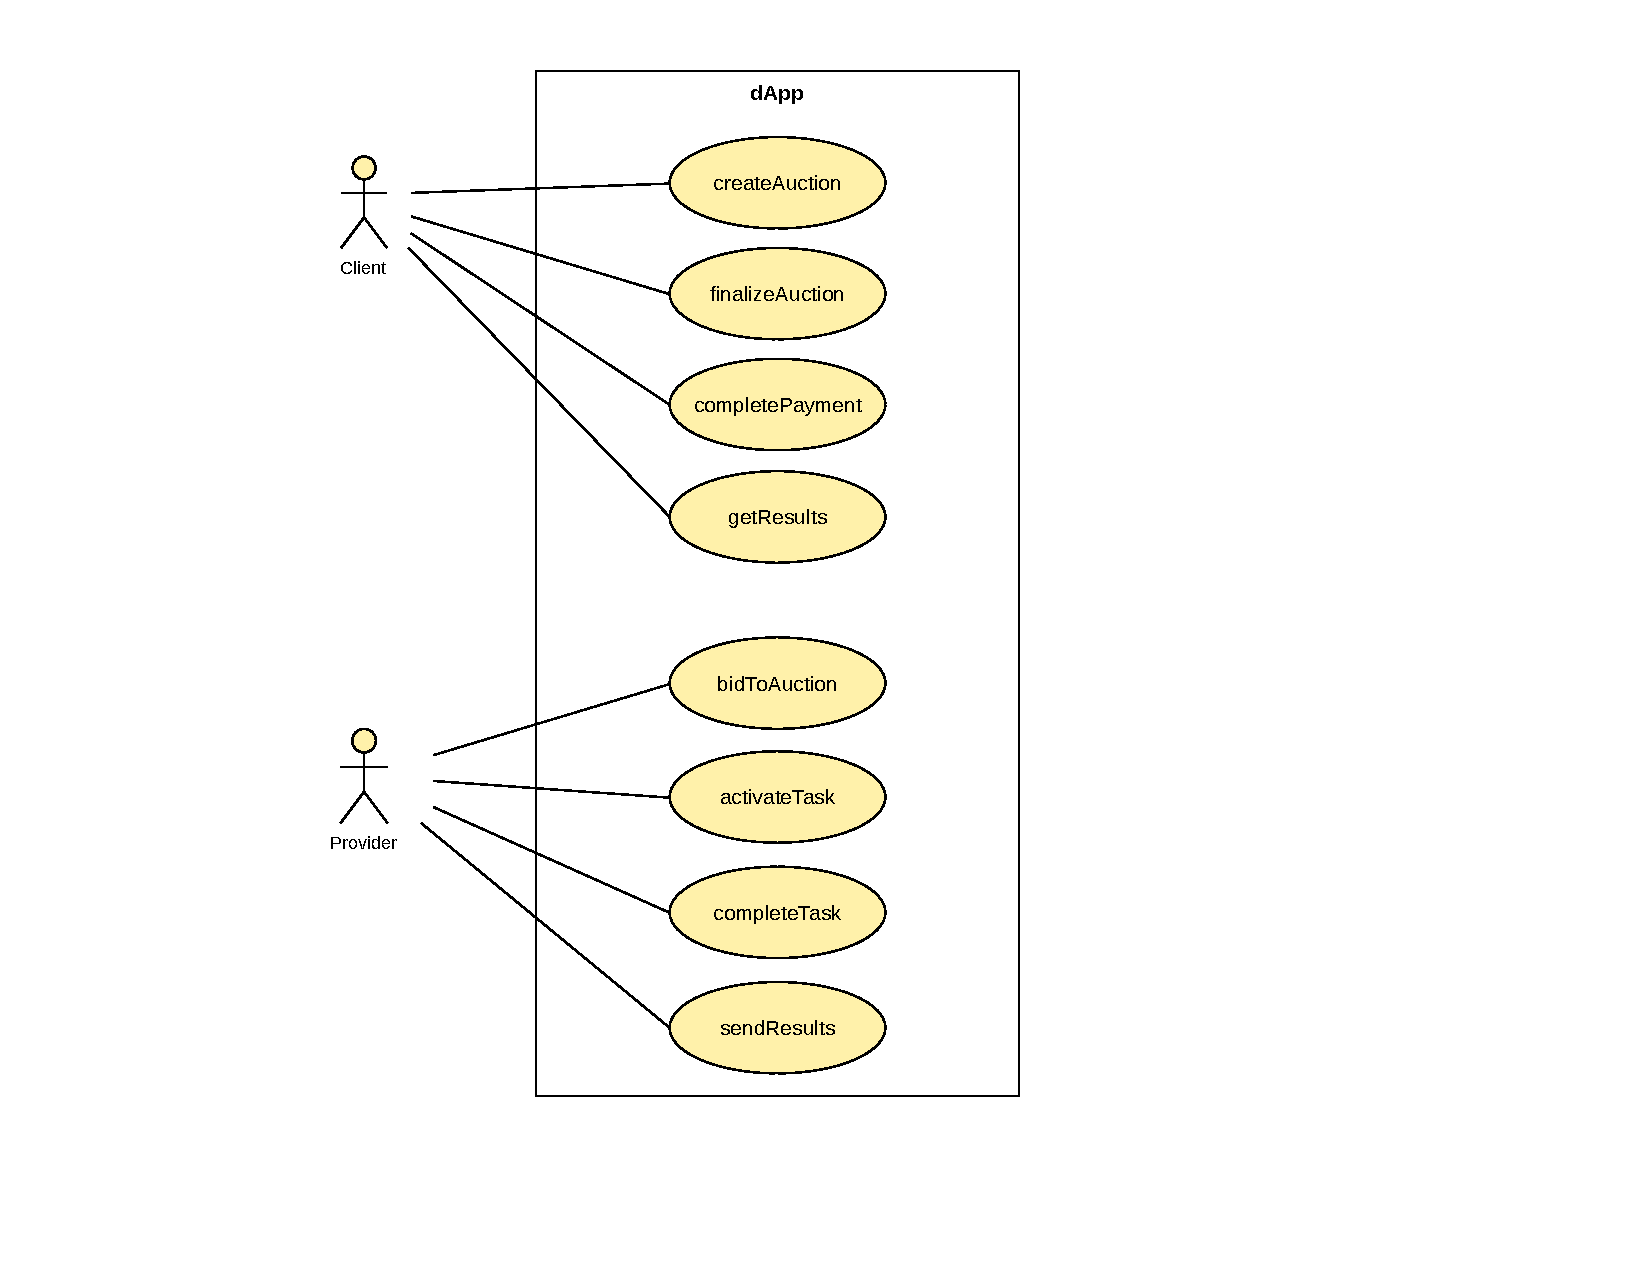
\includegraphics[width=0.5\textwidth]{figures/figure-003.pdf}
    \caption{\en{Use case diagram} της \en{dApp}} 
\end{illustration}

Με σαφή κατανόηση των ρόλων των πελατών και των παρόχων, παρακάτω αναλύεται η τεχνική αρχιτεκτονική που διευκολύνει τις αλληλεπιδράσεις τους και διασφαλίζει την σταθερότητα του συστήματος.

\section{Αρχιτεκτονική του συστήματος}
Η αρχιτεκτονική της \en{dApp} έχει σχεδιαστεί για να διευκολύνει την απρόσκοπτη αλληλεπίδραση μεταξύ πελατών και παρόχων, διασφαλίζοντας παράλληλα την ακεραιότητα και την ασφάλεια των υπολογιστικών εργασιών. 
Ακολουθεί μια ανάλυσή της:
\begin{enumerate}
    \item \en{Smart Contracts}:
        \begin{itemize}
            \item[-] \en{AuctionsManager}: Έξυπνο συμβόλαιο, το οποίο διαχειρίζεται τη διαδικασία δημοπρασίας, από την έναρξή της από τον πελάτη έως την επιλογή ενός παρόχου με βάση τις προσφορές. Χειρίζεται τις προθεσμίες και άλλες παραμέτρους που αφορούν τη δημοπρασία.
            \item[-] \en{TasksManager}: Έξυπνο συμβόλαιο, το οποίο επιβλέπει τον κύκλο ζωής μιας υπολογιστικής εργασίας. Εξασφαλίζει τις διαδικασίες σωστής εκτέλεσης, επαλήθευσης και πληρωμής και διαχειρίζεται επίσης τις χρηματικές εγγυήσεις και τις προθεσμίες που σχετίζονται με κάθε εργασία.
        \end{itemize}
    \item Ενσωμάτωση \en{IPFS}:
        \begin{itemize}
            \item[-] Οι πελάτες μεταφορτώνουν τη μεταγλωττισμένη κλάση \en{Java} (\en{Code.class}) στο \en{IPFS (InterPlanetary FileSystem )} και παρέχουν το \en{CID (Content Identifier)} κατά τη δημιουργία της δημοπρασίας. Αυτό διασφαλίζει ότι ο κώδικας παραμένει αμετάβλητος και προσβάσιμος στον επιλεγμένο πάροχο. 
            \item[-] Οι τυποποιημένες \en{boilerplate} κλάσεις (\en{Main.class} και \en{Time.class}) αποθηκεύονται επίσης στο \en{IPFS} και ανακτώνται χρησιμοποιώντας προκαθορισμένα \en{CID}. 
        \end{itemize}
    \item \en{Docker Container}: 
    \begin{itemize} 
        \item[-] Το \en{Docker  container} χρησιμεύει ως περιβάλλον εκτέλεσης των υπολογιστικών εργασιών. Αποτελείται από δύο πρωταρχικά \en{images}:
        \begin{itemize}
            \item[-] \en{Java Image}: Εκτελεί την \en{Main.class}, η οποία ενορχηστρώνει ολόκληρη τη διαδικασία, από την εκτέλεση της υπολογιστικής εργασίας του πελάτη έως τον υπολογισμό διάρκειάς της και τέλος την εκτύπωση των αποτελεσμάτων.
            \item[-] \en{Node Image}: Μια ειδική ελαφριά έκδοση της \en{dApp} εκτελείται μέσα σε αυτό το \en{docker image}. Αναλύει τα αποτελέσματα από την εκτέλεση της \en{Java class} και τα στέλνει στο έξυπνο συμβόλαιο \en{TasksManager}. Επίσης αποθηκεύει το αποτέλεσμα της εκτέλεσης της εργασίας σε ένα αρχείο στο μηχάνημα του παρόχου ώστε στην συνέχεια να σταλεί στο \en{IPFS} από την \en{dApp}.
        \end{itemize}
    \end{itemize}
    \item Γραφική διεπαφή:
        \begin{itemize}
            \item[-] Κατασκευασμένη με τη χρήση του \en{React Framework}, η διεπαφή της \en{dApp} διευκολύνει τις αλληλεπιδράσεις του χρήστη με το σύστημα. Επιτρέπει στους πελάτες να ξεκινούν δημοπρασίες, στους παρόχους να υποβάλλουν προσφορές και στα δύο μέρη να διαχειρίζονται και να παρακολουθούν τις εργασίες που συμμετέχουν. Η διεπαφή χειρίζεται επίσης τον κατακερματισμό της συμβολοσειράς επαλήθευσης και αλληλεπιδρά με το \en{Ethereum blockchain} μέσω \en{events} που στέλνονται από τα \en{smart contracts}. 
        \end{itemize}
    \item Μηχανισμός επαλήθευσης:
     \begin{itemize}
        \item[-] Όπως αναλύθηκε προηγουμένως, ο μηχανισμός επαλήθευσης διασφαλίζει ότι οι πάροχοι εκτελούν πραγματικά την υπολογιστική εργασία του πελάτη. Η μέθοδος \en{getVerification} στην \en{Code.class} επιστρέφει μια συμβολοσειρά που ορίζεται από τον πελάτη, η οποία, όταν κατακερματιστεί και συγκριθεί με τον αποθηκευμένο κατακερματισμό που δηλώθηκε από τον πελάτη στο συμβόλαιο \en{AuctionsManager}, επαληθεύει την ορθή εκτέλεση της εργασίας.
     \end{itemize}
    \item Σύστημα πληρωμών και εγγυήσεων: 
    \begin{itemize}
        \item[-] Τόσο οι πελάτες όσο και οι πάροχοι τοποθετούν χρηματικές εγγυήσεις για να διασφαλίσουν τη δέσμευσή τους στην εργασία. Μετά την επιτυχή ολοκλήρωση και επαλήθευση της εργασίας, ο πελάτης πληρώνει τον πάροχο με βάση το συμφωνημένο ποσο (\en{wei} ανά δευτερόλεπτο εκτέλεσης) και την διάρκεια της εκτέλεσης. Τα προαναφερθέντα έξυπνα συμβόλαια χειρίζονται αυτές τις συναλλαγές, εξασφαλίζοντας διαφάνεια και ασφάλεια.
    \end{itemize}
\end{enumerate}

\begin{illustration}
    \centering
    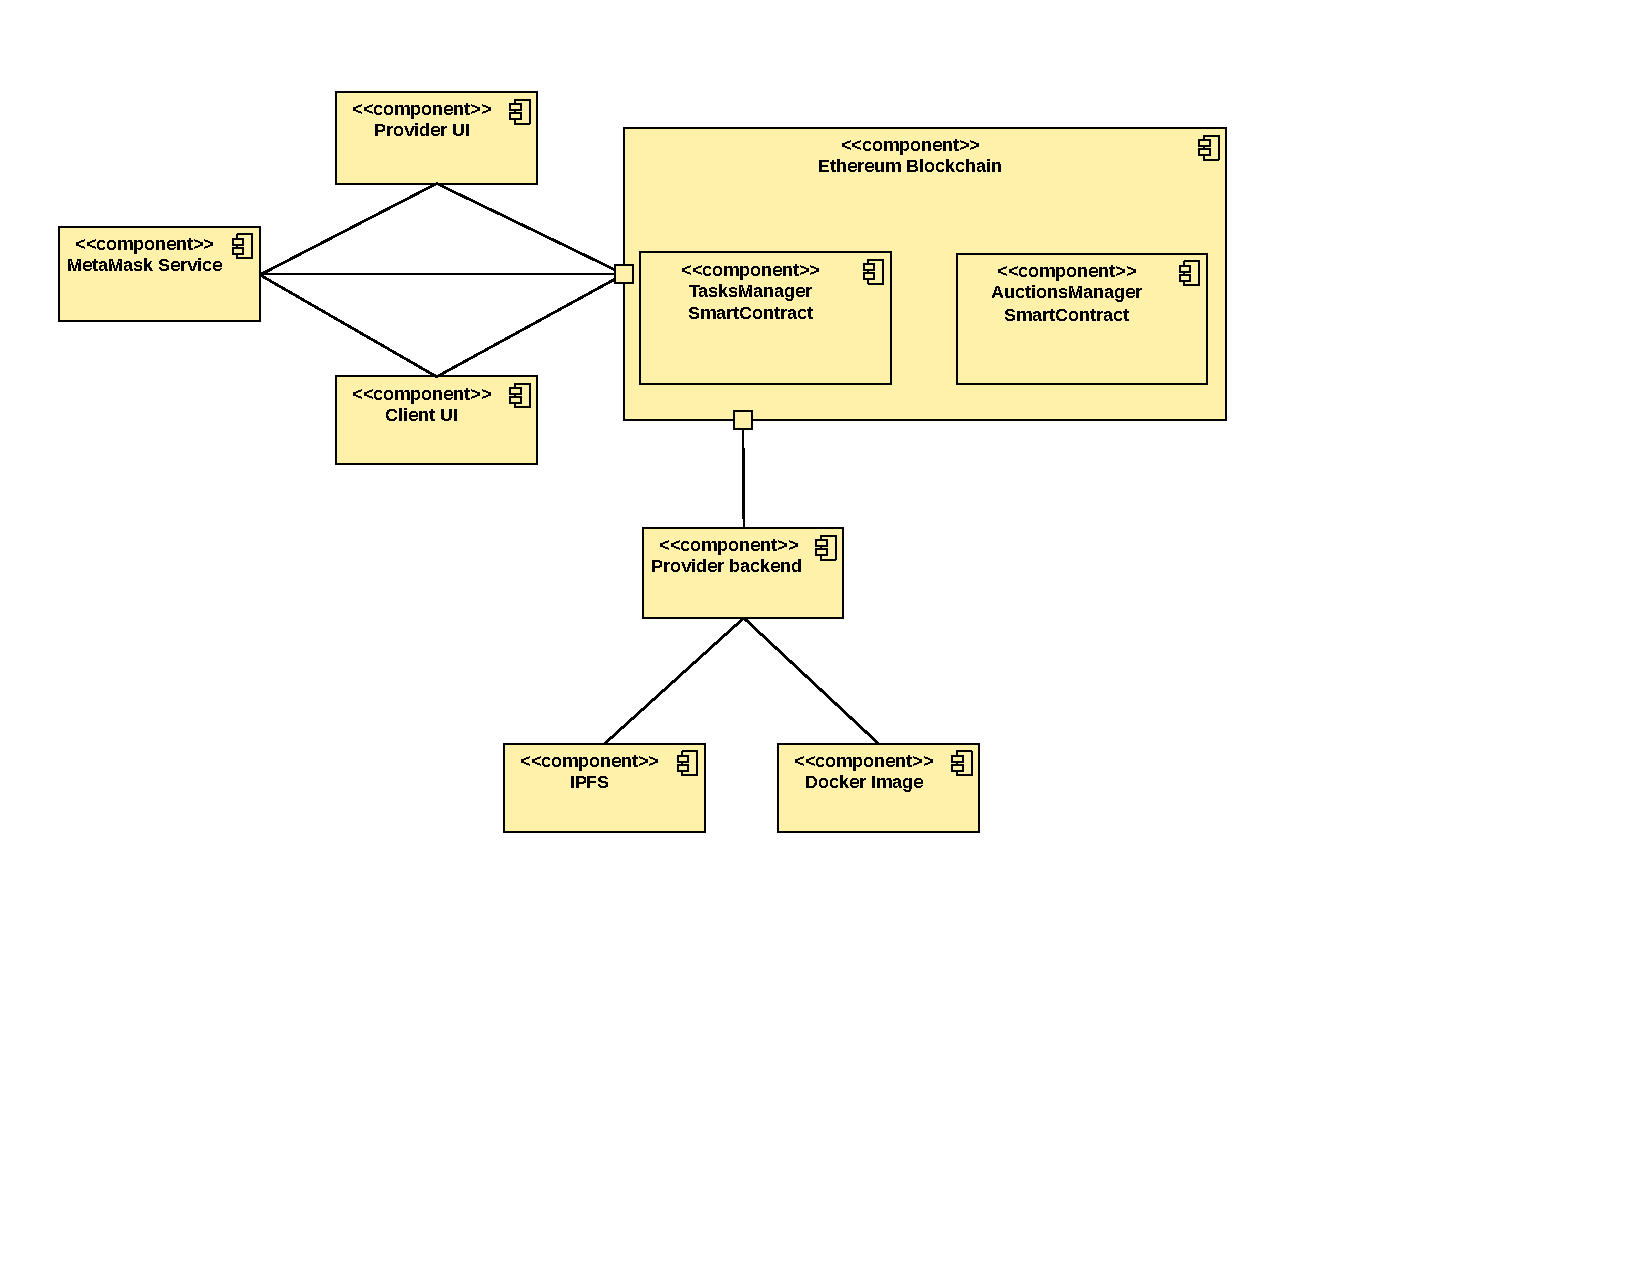
\includegraphics[width=0.8\textwidth]{figures/figure-004.pdf}
    \caption{\en{Component diagram} της \en{dApp}} 
\end{illustration}

Με την ενσωμάτωση αυτών των στοιχείων, η αρχιτεκτονική της \en{dApp} εξασφαλίζει ένα στιβαρό, ασφαλές και αποτελεσματικό σύστημα για αποκεντρωμένο υπολογιστικό νέφος. 

Ο σχεδιασμός δίνει προτεραιότητα στην αξιοπιστία, διασφαλίζοντας ότι τόσο οι πελάτες όσο και οι πάροχοι μπορούν να συμμετέχουν σε υπολογιστικές εργασίες με εμπιστοσύνη.

Η αρχιτεκτονική παρέχει ένα σχέδιο του συστήματος, δίνοντας έμφαση στα συστατικά του 
και στις αλληλεπιδράσεις τους. 

Παρακάτω παρουσιάζεται η συμπεριφορά του συστήματος τόσο στο πρωταρχικό σενάριο εκτέλεσής του, όσο και στα εναλλακτικά μη ιδανικά σενάρια.

\section{Ροές εργασιών του συστήματος}
\subsection{Επιτυχής ολοκλήρωση εργασίας }
Τα βήματα που ακολουθούνται έως την επιτυχή ολοκλήρωση μιας εργασίας είναι τα ακόλουθα:
\begin{enumerate}
    \item Δημιουργία εργασιών: Ο πελάτης γράφει και μεταγλωττίζει την κλάση \en{Java} με το όνομα \textit{\en{Code}}. Η κλάση αυτή περιέχει δύο \en{public} μεθόδους: την \textit{\en{getComputation}} που περιέχει τη λογική της εργασίας και την \textit{\en{getVerification}} που επιστρέφει μια προκαθορισμένη συμβολοσειρά για επαλήθευση. Η κλάση \textit{\en{getComputation}} έχει επιλεγεί να επιστρέφει \en{String} για συμβατότητα της \en{Main.class} με κάθε συνάρτηση υπολογισμού.
    \item \en{IPFS Upload}: Ο πελάτης μεταφορτώνει την μεταγλωττισμένη κλάση του στο \en{IPFS} (\en{InterPlanetary FileSystem}) και λαμβάνει ένα \en{CID} (\en{Content Identifier}).
    \item Έναρξη δημοπρασίας: Χρησιμοποιώντας την \en{dApp}, ο πελάτης ξεκινά μια δημοπρασία, παρέχοντας τις απαραίτητες λεπτομέρειες, όπως η προθεσμία της δημοπρασίας, η προθεσμία εκτέλεσης της εργασίας, το \en{CID} της \en{Java} κλάσης και την συμβολοσειρά επαλήθευσης.
    \item Υποβολή προσφοράς: Οι πάροχοι υποβάλλουν προσφορά για την εργασία καθορίζοντας την τιμή (σε \en{wei} ανά δευτερόλεπτο εκτέλεσης) που προτείνουν.
    \item Επιλογή παρόχου: Ο πελάτης επιλέγει τον πάροχο που επιθυμεί να εκτελέσει την εργασία του, βασιζόμενος στην τιμή προσφοράς και στην βαθμολογία που έχει προκύψει από προηγούμενες επιδόσεις του παρόχου. Στο βήμα αυτό, ο πελάτης στέλνει ως εγγύηση το ποσό που αντιστοιχεί σε 2 δευτερόλεπτα εκτέλεσης της εργασίας.
    \item Ενεργοποίηση της εργασίας: Ο πάροχος ενεργοποιεί την εργασία στέλνοντας την δική του εγγύηση, η οποία αντιστοιχεί σε 10 δευτερόλεπτα εκτέλεσης της εργασίας. Στην συνέχεια, το \en{dApp} ενορχηστρώνει την διαδικασία εκτέλεσης της εργασίας, λαμβάνοντας από το \en{IPFS} τις απαραίτητες κλάσεις, δημιουργώντας την εικόνα \textit{\en{Docker}} και εκκινώντας τον \en{docker container}.
    \item Εκτέλεση εργασίας: Εντός του \en{docker container}, εκτελείται η κλάση \en{Java}. Η συμβολοσειρά επαλήθευσης, μαζί με την διάρκεια εκτέλεσης και τον χρόνο ολοκλήρωσης της εργασίας στέλνονται στο \en{smart contract} \textit{\en{TasksManager}} για τον έλεγχο της διαδικασίας. Τα αποτελέσματα του υπολογισμού εγγράφονται σε ένα αρχείου κειμένου. Το συμβόλαιο επαληθεύει την ορθή εκτέλεση της εργασίας με βάση την παρεχόμενη συμβολοσειρά επαλήθευσης και διασφαλίζει ότι ολοκληρώθηκε εντός της συμφωνημένης προθεσμίας. Στην περίπτωση ορθής και έγκαιρης εκτέλεσης, η βαθμολογία του παρόχου αυξάνεται και οι χρηματικές εγγυήσεις του επιστρέφονται.
    \item Υποβολή αποτελέσματος: To \en{dApp} μεταφορτώνει εκ μέρους του παρόχου το αποτέλεσμα της εργασίας στο \en{IPFS} και υποβάλλει το \en{CID} στο \en{smart contract} \textit{\en{TasksManager}}.
    \item Πληρωμή: Μετά την επιτυχή εκτέλεση και υποβολή των αποτελεσμάτων από τον πάροχο, ο πελάτης ενημερώνεται για το ποσό που οφείλει να πληρώσει, με βάση την διάρκεια εκτέλεσης της εργασίας. Στην συνέχεια αποστέλλει στο \en{smart contract} \textit{\en{TasksManager}} το ποσό της πληρωμής που εκκρεμεί και τότε μπορεί να αποκτήσει πρόσβαση στο \en{CID} των αποτελεσμάτων. Με την επιτυχημένη ολοκλήρωση της πληρωμής η βαθμολογία του πελάτη αυξάνεται, ως δείκτης φερεγγυότητας.
\end{enumerate}

\subsection{Εναλλακτικές ροές εργασιών}
\subsubsection{Ανεπιτυχής ολοκλήρωση της εργασίας λόγω ασυμφωνίας επαλήθευσης \\ή καθυστερημένης εκτέλεσης}
Κατά τη λήψη των αποτελεσμάτων από τον πάροχο, το \en{smart contract TasksManager} κατακερματίζει και ελέγχει την συμβολοσειρά επαλήθευσης.
Εάν η κατακερματισμένη συμβολοσειρά επαλήθευσης δεν ταιριάζει με αυτήν που παρέχεται από τον πελάτη, η εργασία θεωρείται ανεπιτυχής.

Ταυτόχρονα, ελέγχεται και ο χρόνος ολοκλήρωσης της εκτέλεσης. Εάν η εργασία ολοκληρώθηκε μετά τη συμφωνηθείσα προθεσμία, θεωρείται επίσης ανεπιτυχής.

Και στις δύο περιπτώσεις ανεπιτυχούς επαλήθευσης ή καθυστερημένης εκτέλεσης, η βαθμολογία του παρόχου μειώνεται, ενώ οι χρηματικές εγγυήσεις του χάνονται και παραμένουν στο έξυπνο συμβόλαιο \en{TasksManager}. Στον πελάτη επιστρέφονται οι δικές του χρηματικές εγγυήσεις.

\subsubsection{Καθυστέρηση του παρόχου στην υποβολή των αποτελεσμάτων}
Μετά την επιτυχημένη εκτέλεση της εργασίας, ο πάροχος έχει περιθώριο μίας ημέρας για να υποβάλει τα αποτελέσματα στο έξυπνο συμβόλαιο \en{TasksManager}. Εάν ο πάροχος δεν υποβάλει τα αποτελέσματα εντός αυτού του χρονικού διαστήματος, η βαθμολογείται αρνητικά και χάνει τις χρηματικές εγγυήσεις του, οι οποίες παραμένουν στο συμβόλαιο. Παράλληλα, επιστρέφονται στον πελάτη οι δικές του χρηματικές εγγυήσεις.

\subsubsection{Δικαίωμα ακύρωσης του πελάτη πριν από την ενεργοποίηση της \\εργασίας}
Μέχρι ο πάροχος να ενεργοποιήσει την υπολογιστική εργασία, ο πελάτης έχει το δικαίωμα να την ακυρώσει. Κατά την ακύρωση, οι εξασφαλίσεις του πελάτη επιστρέφονται. Στο βήμα αυτό ο πάροχος δεν έχει αποστείλει ακόμα τις δικές του χρηματικές εγγυήσεις ώστε να του επιστραφούν.

\subsubsection{Δικαίωμα ακύρωσης του πελάτη για καθυστερημένη ολοκλήρωση}
Στην περίπτωση που έχει παρέλθει ο χρόνος της προσυμφωνημένης προθεσμίας για την εκτέλεση της υπολογιστικής εργασίας, δίνοντας ακόμη περιθώριο μιας ημέρας, ο πελάτης έχει το δικαίωμα να ακυρώσει την εργασία. Στην περίπτωση αυτή, μεταφέρεται στον πελάτη τόσο η δική του χρηματική εγγύηση, όσο και του παρόχου. 

\subsubsection{Μη ολοκλήρωση πληρωμής από τον πελάτη}
Στην περίπτωση επιτυχημένης εκτέλεσης της εργασίας εκ μέρους του παρόχου, ο πελάτης έχει το περιθώριο μιας ημέρας για να ολοκληρώσει την πληρωμή. Αν αυτό δεν συμβεί, ο πάροχος έχει το δικαίωμα να τον καταγγείλει. Τότε η βαθμολογία του πελάτη μειώνεται, ως δείγμα αφερεγγυότητας. \\

Παρακάτω παρουσιάζεται το \en{Activity Diagram} της \en{dApp} για τις βασικές ροές εκτέλεσής της.
\begin{illustration}
    \centering
    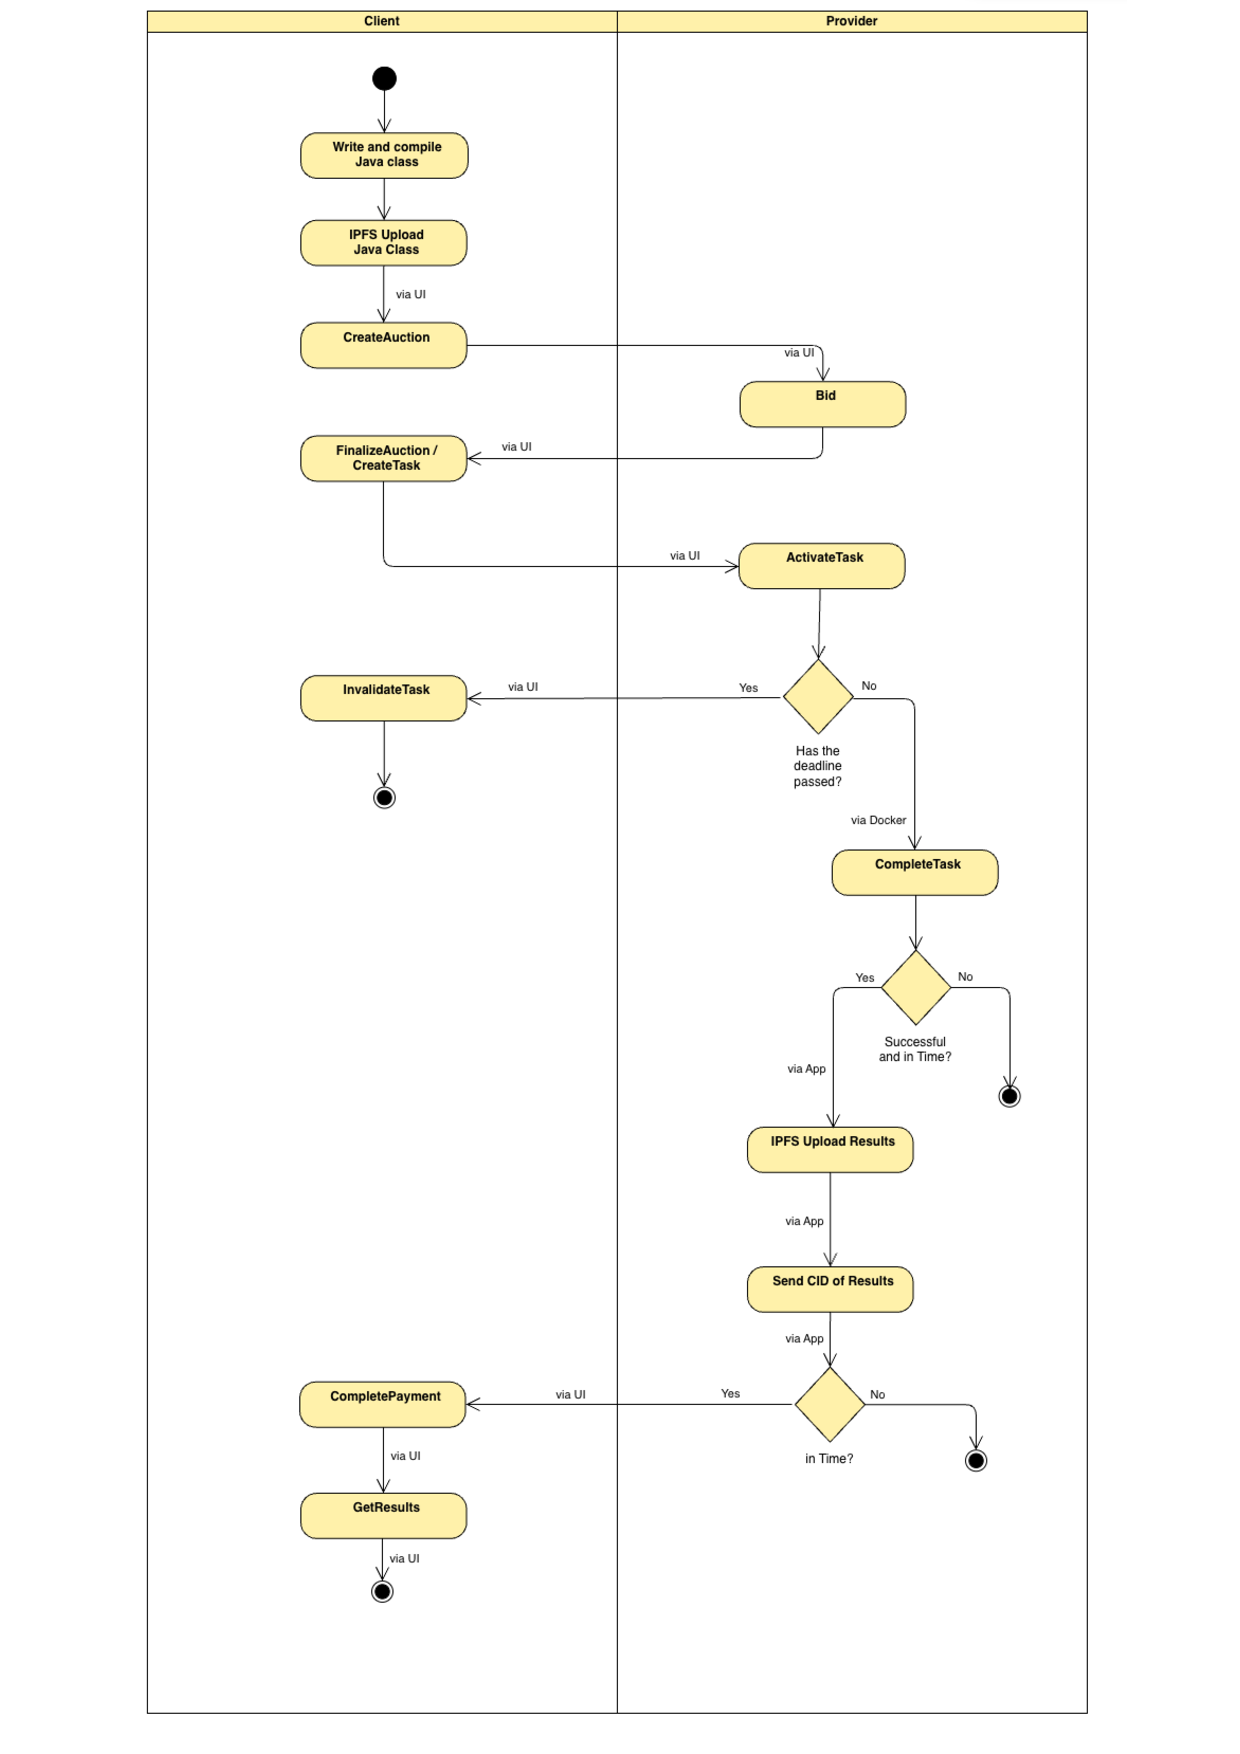
\includegraphics[width=1.1\textwidth]{figures/figure-005.pdf}
    \caption{\en{Activity diagram} της \en{dApp}} 
\end{illustration}

\newpage
Ενώ οι εναλλακτικές ροές εξασφαλίζουν ευελιξία και ευρωστία σε διάφορα σενάρια, το θεμέλιο αυτής της \en{dApp} έγκειται στα μέτρα ασφαλείας της. Τα μέτρα αυτά όχι μόνο προστατεύουν τα συμφέροντα των πελατών και των παρόχων, αλλά διασφαλίζουν επίσης τη συνολική αξιοπιστία του συστήματος. 

Παρακάτω παρουσιάζονται οι μηχανισμοί ασφάλειας της \en{dApp}.


\section{Μέτρα ασφαλείας για τη διασφάλιση της αξιοπιστίας}
Η αξιοπιστία του συστήματος διασφαλίζεται εφαρμόζοντας τα ακόλουθα μέτρα:
\begin{itemize}
\item[-] Συμβολοσειρά επαλήθευσης: Ο πελάτης παρέχει μια συμβολοσειρά επαλήθευσης που επιθυμεί, η οποία κατακερματίζεται (πραγματοποιείται \en{hash} με τον αλγόριθμο \en{keccak256} που χρησιμοποιεί το \en{Ethereum virtual machine}) και αποθηκεύεται στο έξυπνο συμβόλαιο. Αυτό διασφαλίζει ότι ο πάροχος έχει εκτελέσει πραγματικά την εργασία, καθώς για την επαλήθευση πρέπει να επιστρέψει στο συμβόλαιο την σωστή συμβολοσειρά στην αρχική της μορφή (πριν κατακερματιστεί) χωρίς να έχει άμεση πρόσβαση σε αυτή.
\item[-] \en{Docker containerization}: Για να διασφαλιστεί η ασφάλεια του μηχανήματος του παρόχου και να αποτραπεί η αλλοίωση της εκτέλεσης από αυτόν, οι εργασίες εκτελούνται σε \en{docker containers}. Η ενθυλάκωση αυτή εξασφαλίζει ένα συνεπές και απομονωμένο περιβάλλον για την εκτέλεση των εργασιών.
\item[-] \en{Blockchain}: Όλες οι αλληλεπιδράσεις, από την έναρξη της δημοπρασίας έως την ολοκλήρωση της εργασίας, καταγράφονται στο \en{Blockchain}. Αυτό διασφαλίζει τη διαφάνεια και επιτρέπει στους ενδιαφερόμενους να επαληθεύουν όλες τις ενέργειες. 
\item[-] Μηχανισμός εγγυήσεων:  Τόσο ο πελάτης όσο και ο πάροχος αποστέλλουν χρηματικές εγγυήσεις στο έξυπνο συμβόλαιο. Αυτό λειτουργεί ως δέσμευση και διασφαλίζει ότι και τα δύο μέρη ενεργούν με ειλικρίνεια και έχουν κίνητρο για την επιτυχή ολοκλήρωση της διαδικασίας, καθώς σε περίπτωση ασυμφωνίας στην οποία ευθύνονται μπορεί να χάσουν τις εγγυήσεις τους. 
\item[-] Επικοινωνία μέσω \en{events}: Η \en{dApp} και τα έξυπνα συμβόλαια επικοινωνούν μέσω \en{events} που παρέχουν τα συμβόλαια. Αυτό διασφαλίζει ότι όλα τα ενδιαφερόμενα μέρη ενημερώνονται άμεσα για τα διάφορα στάδια του κύκλου ζωής της εργασίας. 
\end{itemize}

Με την ενσωμάτωση αυτών των μέτρων ασφαλείας, η \en{dApp} διασφαλίζει ένα αξιόπιστο περιβάλλον τόσο για τους πελάτες όσο και για τους παρόχους, προωθώντας τη δίκαιη και διαφανή εκτέλεση των υπολογιστικών εργασιών.
	\chapter{Μηχανισμός δημοπρασίας}
\InitialCharacter{Ο} μηχανισμός δημοπρασίας χρησιμεύει ως ο ακρογωνιαίος λίθος της προτεινόμενης αποκεντρωμένης εφαρμογής (\en{dApp}), δημιουργώντας μια διαφανή και δίκαιη πλατφόρμα για την κατανομή των υπολογιστικών εργασιών. Η παρούσα ενότητα διευκρινίζει την περίπλοκη δυναμική της διαδικασίας δημοπρασίας, τις στρατηγικές υποβολής προσφορών που χρησιμοποιούν οι πάροχοι και τα πολύπλευρα κριτήρια που καθοδηγούν την επιλογή ενός παρόχου από έναν πελάτη.

\section{Επισκόπηση της διαδικασίας δημοπρασίας}
Η διαδικασία δημοπρασίας ξεκινά όταν ένας πελάτης υποβάλλει μια υπολογιστική εργασία στην \en{dApp}. Η διαδικασία αυτή είναι δομημένη ώστε να διασφαλίζεται η δικαιοσύνη, η διαφάνεια και η βέλτιστη κατανομή εργασιών:
\begin{enumerate}
    \item Υποβολή εργασίας: Οι πελάτες ξεκινούν τη δημοπρασία αναφέροντας τις λεπτομέρειες της υπολογιστικής εργασίας και συγκεκριμένα την αναμενόμενη προθεσμία ολοκλήρωσης και τη σχετική συμβολοσειρά επαλήθευσης.
    \item Υποβολή προσφορών: Μετά την υποβολή της εργασίας, οι πάροχοι έχουν την ευκαιρία να εξετάσουν τις λεπτομέρειες της εργασίας και να υποβάλλουν τις προσφορές τους με την προτεινόμενη τιμή τους (σε \en{wei} ανά δευτερόλεπτο εκτέλεσης της εργασίας).
    \item Επιλογή παρόχου: Όσο η δημοπρασία παραμένει ενεργή, ο πελάτης μπορεί να επιλέξει τον πάροχο που επιθυμεί, βασιζόμενος σε διάφορους παράγοντες που θα αναλυθούν παρακάτω. Η απόφαση αυτή σηματοδοτεί την ολοκλήρωση της δημοπρασίας και την έναρξη της φάσης εκτέλεσης της εργασίας.
\end{enumerate}

\section{Μηχανισμός βαθμολόγησης}
Στο \en{smart contract} \en{TasksManager} αποθηκεύεται το ιστορικό των επιδόσεων των παρόχων και των πελατών στην διαδικασία μέσω ενός μηχανισμού βαθμολόγησης. Ο μηχανισμός αυτός είναι καθοριστικής σημασίας για τη διατήρηση της ακεραιότητας της \en{dApp}, διασφαλίζοντας ότι τόσο οι πάροχοι όσο και οι πελάτες λογοδοτούν για τις πράξεις και τις επιδόσεις τους.
\begin{itemize}
    \item Βαθμολογία του παρόχου: Σε κάθε πάροχο αποδίδεται μια βαθμολογία, η οποία προκύπτει από τον συνδυασμό των ανεπιτυχών (\en{downVotes}) και επιτυχών (\en{upVotes}) εκτελέσεων εργασιών, η οποία αντικατοπτρίζει το ιστορικό των επιδόσεων τους. Ο υπολογισμός της βαθμολογίας χρησιμοποιεί τη μεθοδολογία "ταξινόμησης εμπιστοσύνης" που βασίζεται στο διάστημα βαθμολογίας \en{Wilson}, έναν διάσημο αλγόριθμο που χρησιμοποιείται από πλατφόρμες όπως το \en{Reddit} για την ταξινόμηση των σχολίων στην πλατφόρμα. Με τον τρόπο αυτό διασφαλίζεται ότι η βαθμολογία δεν είναι απλώς ένας μέσος όρος, αλλά μια αναπαράσταση της αξιοπιστίας του παρόχου με βάση τον όγκο και την αναλογία των \en{upvotes} προς τα \en{downvotes} του. 
    \item Βαθμολογία πελάτη: Στους πελάτες αποδίδεται επίσης μια αντίστοιχη βαθμολογία, ενδεικτική των ιστορικών αλληλεπιδράσεών τους και της συνέπειάς τους στην αμοιβή των παρόχων για επιτυχώς εκτελεσμένες εργασίες. Η βαθμολογία αυτή παίζει καθοριστικό ρόλο στη διαμόρφωση της στρατηγικής προσφορών του παρόχου.
\end{itemize}

\section{Κριτήρια που καθοδηγούν τον πελάτη στην επιλογή \\παρόχου}
Η επιλογή του παρόχου από τον πελάτη επηρεάζεται από μια σειρά παραγόντων, διασφαλίζοντας ότι η απόφαση είναι τόσο τεκμηριωμένη όσο και βέλτιστη:
\begin{itemize}
    \item Προσφορά τιμής: Η προτεινόμενη τιμή του παρόχου παραμένει πρωταρχικής σημασίας, με τους πελάτες να κλίνουν φυσικά προς τις ανταγωνιστικές τιμές.
    \item Το ιστορικό επιδόσεων του παρόχου: Η βαθμολογία του παρόχου, όπως υπολογίζεται με την προαναφερθείσα μεθοδολογία, προσφέρει πληροφορίες σχετικά με την αξιοπιστία και τις προηγούμενες επιδόσεις του.
    \item Προηγούμενες συνεργασίες: Προηγούμενες συνεργασίες με τον συγκεκριμένο πάροχο που κατέληξαν σε θετικά αποτελέσματα μπορούν να επηρεάσουν σημαντικά την απόφαση ενός πελάτη.
\end{itemize}

\section{Παράγοντες που διαμορφώνουν τη στρατηγική προσφορών του παρόχου}
Οι πάροχοι, κατά τη διαμόρφωση των προσφορών τους, εξετάζουν πληθώρα παραγόντων για να βελτιστοποιήσουν τις πιθανότητές τους να επιλεγούν, εξασφαλίζοντας παράλληλα την κερδοφορία τους:
\begin{itemize}
    \item Η αξιοπιστία του πελάτη: Η βαθμολογία ενός πελάτη, ενδεικτική των προηγούμενων αλληλεπιδράσεών του και της συνέπειας των πληρωμών του, μπορεί να επηρεάσει το ποσό της προσφοράς του παρόχου.
    \item Διαθεσιμότητα πόρων του παρόχου: Οι πάροχοι με άφθονους πόρους ενδέχεται να έχουν την προδιάθεση να υποβάλουν χαμηλότερη προσφορά για να εξασφαλίσουν την εργασία.
    \item Ιστορικό αλληλεπιδράσεων με τον πελάτη: Οι θετικές αλληλεπιδράσεις του παρελθόντος με τον πελάτη μπορούν να παρακινήσουν έναν πάροχο να υποβάλει μια πιο ανταγωνιστική προσφορά.
\end{itemize}

Συνοψίζοντας, ο μηχανισμός δημοπρασίας, ο οποίος υποστηρίζεται από τη διαφανή διαδικασία υποβολής προσφορών, τα κριτήρια αξιολόγησης και το σύστημα βαθμολόγησης, ενισχύει τη δέσμευση της \en{dApp} για την προώθηση ενός αξιόπιστου και αποτελεσματικού περιβάλλοντος για την αποκεντρωμένη εφαρμογή υπολογιστικής νέφους.

	\chapter{Εκτέλεση εργασίας και επαλήθευση}
\InitialCharacter{Τ} ο στάδιο εκτέλεσης και επαλήθευσης της εργασίας είναι κομβικής σημασίας στην αποκεντρωμένη εφαρμογή (\en{dApp}), διασφαλίζοντας ότι οι υπολογιστικές εργασίες όχι μόνο εκτελούνται με ακρίβεια και αποτελεσματικότητα από τον επιλεγμένο πάροχο, αλλά και ότι τα αποτελέσματα είναι επαληθεύσιμα και γνήσια. Αυτό το κεφάλαιο εμβαθύνει στις ιδιαιτερότητες της εκτέλεσης εργασιών, στον μηχανισμό που χρησιμοποιείται για την επαλήθευση της ορθότητας της εκτέλεσης και στην ασφαλή και διαφανή διαδικασία πληρωμής που διευκολύνεται από την τεχνολογία \en{blockchain}.


\section{Εκτέλεση εργασιών}
Η εκτέλεση μιας υπολογιστικής εργασίας είναι μια σχολαστική διαδικασία, η οποία διασφαλίζει ότι ο πάροχος τηρεί τις προκαθορισμένες απαιτήσεις και εκτελεί την εργασία εντός του καθορισμένου περιβάλλοντος.
\begin{enumerate}
    \item Ενεργοποίηση της εργασίας: Μετά την επιλογή του από τον πελάτη, ο πάροχος ενεργοποιεί την εργασία, σηματοδοτώντας τη δέσμευσή του για την εκτέλεσή της. Στα πλαίσια της δέσμευσης αυτής, στο σημείο αυτό στέλνει στο συμβόλαιο χρηματική εγγύηση ίση με την αξία εκτέλεσης της εργασίας για 2 δευτερόλεπτα.
    \item Περιβάλλον απομόνωσης: Για να διασφαλιστεί το σύστημα του παρόχου και να εξασφαλιστεί ένα συνεπές περιβάλλον εκτέλεσης, οι εργασίες εκτελούνται εντός \en{Docker container}. Αυτή η ενθυλάκωση απομονώνει την εκτέλεση από εξωτερικές παρεμβάσεις και πιθανές απειλές ασφαλείας.
    \item Ανάκτηση κώδικα: Ο πάροχος ανακτά τη μεταγλωττισμένη κλάση \en{Java} του πελάτη από το \en{IPFS} χρησιμοποιώντας το \en{CID} της.
    \item Εκτέλεση εργασιών: Εντός του \en{Docker container}, η κλάση \en{Java} εκτελείται, τηρώντας τη λογική που περιέχεται στη μέθοδο \textit{\en{getComputation}} από τον πελάτη.
    \item Αποστολή αποτελεσμάτων: Τα αποτελέσματα εκτέλεσης της υπολογιστικής εργασίας αποθηκεύονται σε ένα αρχείο, μεταφορτώνονται στο \en{IPFS} και το \en{CID} τους αποστέλλεται στο \en{smart contract} ώστε να το λάβει ο πελάτης μετά την ολοκλήρωση της πληρωμής του.
\end{enumerate}

\section{Μηχανισμός επαλήθευσης}
Η διασφάλιση της πραγματικής εκτέλεσης της εργασίας είναι καθοριστικής σημασίας και η \en{dApp} χρησιμοποιεί έναν ισχυρό μηχανισμό επαλήθευσης για να εξακριβώσει τη γνησιότητα των αποτελεσμάτων.

\begin{enumerate}
    \item Συμβολοσειρά επαλήθευσης: Η μέθοδος \textit{\en{getVerification}} εντός της εκτελούμενης κλάσης \en{Java} επιστρέφει μια προκαθορισμένη συμβολοσειρά, η οποία είναι άγνωστη στον πάροχο.
    \item Σύγκριση κατακερματισμένης συμβολοσειράς: Η επιστρεφόμενη συμβολοσειρά επαλήθευσης κατακερματίζεται και συγκρίνεται με τον αρχικό κατακερματισμό που δόθηκε από τον πελάτη κατά την έναρξη της δημοπρασίας.
    \item Επικύρωση αποτελέσματος: Εάν οι κατακερματισμένες συμβολοσειρές ταιριάζουν, το αποτέλεσμα θεωρείται γνήσιο και η εργασία κρίνεται επιτυχημένη.
    Αντίθετα, μια αναντιστοιχία υποδηλώνει ασυμφωνία, ενεργοποιώντας την ανεπιτυχή ροή της εργασίας.
    \item Επαλήθευση χρόνου: Επιπλέον, ο χρόνος εκτέλεσης επαληθεύεται σε σχέση με τη συμφωνηθείσα προθεσμία, ώστε να διασφαλιστεί η έγκαιρη ολοκλήρωση της εργασίας.
\end{enumerate}

\section{Διαδικασία πληρωμής}
Μετά την επιτυχή επαλήθευση, ξεκινά η διαδικασία πληρωμής, διασφαλίζοντας μια διαφανή συναλλαγή μεταξύ του πελάτη και του παρόχου.

\begin{enumerate}
    \item Υπολογισμός πληρωμής: Το ποσό πληρωμής υπολογίζεται με βάση τη συμφωνηθείσα τιμή (\en{wei} ανά δευτερόλεπτο) και τον πραγματικό χρόνο εκτέλεσης. Από αυτό αφαιρείται το ποσό που έχει ήδη στείλει στο συμβόλαιο ο πελάτης ως χρηματική εγγύηση.
    \item Συναλλαγή \en{blockchain}: Η πληρωμή πραγματοποιείται μέσω του έξυπνου συμβολαίου \en{TasksManager} στο \en{Ethereum  blockchain}, εξασφαλίζοντας ασφάλεια και διαφάνεια.
    \item Χειρισμός εγγυήσεων: Μετά την επιτυχή εκτέλεση της εργασίας, επιστρέφονται στον πάροχο οι χρηματικές εγγυήσεις που είχε αποστείλει κατά την έναρξη της διαδικασίας. Σε περιπτώσεις ανεπιτυχούς εκτέλεσης της εργασίας, οι χρηματικές εγγυήσεις του υπεύθυνου χάνονται, όπως περιγράφεται λεπτομερώς στο προηγούμενο κεφάλαιο.
\end{enumerate}

\section{Ασφάλεια κατά την εκτέλεση και την πληρωμή}
Η \en{dApp} διακατέχεται από διάφορα μέτρα ασφαλείας για τη διασφάλιση των συμφερόντων τόσο των πελατών όσο και των παρόχων κατά την εκτέλεση και την πληρωμή.
\begin{itemize}
    \item[-] Αμετάβλητες λεπτομέρειες εργασιών: Οι λεπτομέρειες των εργασιών, αφού μεταφορτωθούν στο \en{IPFS}, είναι αμετάβλητες, διασφαλίζοντας ότι η εκτέλεση τηρεί τις αρχικές απαιτήσεις.
    \item[-] Απομονωμένο περιβάλλον εκτέλεσης: Το \en{Docker container} διασφαλίζει ότι το σύστημα του παρόχου παραμένει απομονωμένο από πιθανό κακόβουλο κώδικα και ότι το περιβάλλον εκτέλεσης είναι συνεπές. 
    \item[-] Διαφανείς συναλλαγές: Όλες οι συναλλαγές, συμπεριλαμβανομένων των πληρωμών και των τοποθετήσεων εγγυήσεων, καταγράφονται στο \en{blockchain}, εξασφαλίζοντας διαφάνεια και επαληθευσιμότητα.
    \item[-] Μηχανισμός εγγυήσεων:  Ο μηχανισμός εγγυήσεων διασφαλίζει τη δέσμευση και των δύο μερών και χρησιμεύει ως αποτρεπτικός παράγοντας έναντι κακόβουλων δραστηριοτήτων ή μη συμμόρφωσης.
\end{itemize}


Ανακεφαλαιώνοντας, το στάδιο εκτέλεσης και επαλήθευσης των εργασιών είναι σχολαστικά σχεδιασμένο ώστε να διασφαλίζεται ότι οι εργασίες εκτελούνται με ακρίβεια, τα αποτελέσματα είναι επαληθεύσιμα και οι πληρωμές είναι ασφαλείς και διαφανείς. Αυτή η φάση, η οποία υποστηρίζεται από την τεχνολογία \en{blockchain} και τους μηχανισμούς που περιγράφηκαν, ενισχύει την αξιοπιστία της \en{dApp} στο αποκεντρωμένο υπολογιστικό νέφος.

	\chapter{Υλοποίηση του συστήματος}
\InitialCharacter{H} ανάπτυξη της αποκεντρωμένης εφαρμογής (\en{dApp}) περιλαμβάνει ένα συνδυασμό τεχνολογιών αιχμής και καινοτόμων λύσεων για την αντιμετώπιση των προκλήσεων του αποκεντρωμένου υπολογιστικού νέφους. Αυτό το κεφάλαιο εμβαθύνει στις τεχνικές ιδιαιτερότητες της \en{dApp}, τα εργαλεία και τις πλατφόρμες που χρησιμοποιήθηκαν και τις προκλήσεις που αντιμετωπίστηκαν κατά την ανάπτυξή της.

\section{Τεχνικές ιδιαιτερότητες της \en{dApp}}
Η αρχιτεκτονική της \en{dApp} συνδυάζει την τεχνολογία του \en{Blockchain}, του \en{containerization} και των κατανεμημένων συστημάτων αρχείων, εξασφαλίζοντας ένα αποτελεσματικό και ασφαλές σύστημα.

\begin{enumerate}
    \item Έξυπνα συμβόλαια: Αναπτυγμένα με τη χρήση της \en{Solidity}, τα έξυπνα συμβόλαια \en{AuctionsManager} και \en{TasksManager} αναπτύσσονται στα \en{blockchains} \en{Ethereum} και \en{Polygon}. Διαχειρίζονται τη διαδικασία δημοπρασίας, τον κύκλο ζωής των εργασιών, τις πληρωμές και τα χρηματικές εγγυήσεις.
    \item Ενσωμάτωση του \en{IPFS}: Το Διαπλανητικό Σύστημα Αρχείων (\en{IPFS}) είναι ένα αποκεντρωμένο σύστημα αποθήκευσης, με βάση την διεύθυνση του περιεχομένου, το οποίο διανέμει αποθηκευμένα αρχεία μεταξύ ομότιμων χρηστών σε ένα δίκτυο \en{P2P}. Το περιεχόμενο κάθε αρχείου κατακερματίζεται και ο κατακερματισμός αυτός \en{(Content Identifier - CID)} χρησιμοποιείται για την ταυτοποίηση και ανάκτηση του συγκεκριμένου αρχείου \cite{ref42}.
    Το σύστημα της εργασίας χρησιμοποιεί το \en{IPFS} για την αποθήκευση και ανάκτηση των μεταγλωττισμένων κλάσεων \en{Java} και των αποτελεσμάτων της εκτέλεσης. Αυτό διασφαλίζει την αμεταβλητότητα των δεδομένων και την αποκεντρωμένη πρόσβαση.
    \item \en{Docker Containerization}: Το \en{Docker} χρησιμοποιείται για τη δημιουργία απομονωμένων περιβαλλόντων για την εκτέλεση εργασιών, εξασφαλίζοντας σταθερή απόδοση και ασφάλεια έναντι πιθανών απειλών.
    \item Γραφική διεπαφή της εφαρμογής: Αναπτυγμένη με τη χρήση του \en{React}, η γραφική διεπαφή διευκολύνει τις αλληλεπιδράσεις του χρήστη, από την έναρξη δημοπρασίας έως την παρακολούθηση εργασιών.
\end{enumerate}

\section{Εργαλεία, γλώσσες προγραμματισμού και πλατφόρμες ανάπτυξης}
Για την ανάπτυξη της \en{dApp} αξιοποιήθηκε πλήθος εργαλείων και πλατφορμών με σκοπό την βέλτιστη απόδοση και εμπειρία των χρηστών.

\begin{enumerate}
    \item Γλώσσες προγραμματισμού
    \begin{itemize}
        \item[-] \en{Solidity}: Για την ανάπτυξη έξυπνων συμβολαίων στο \en{blockchain} του \en{Ethereum} και του \en{Polygon}. 
        \item[-] \en{Java}: Για την υλοποίηση της υπολογιστικής εργασίας τους πελάτη.
        \item[-] \en{Javascript}: Για την γραφική διεπαφή (\en{frontend}) της \en{dApp}.
        \item[-] \en{Typescript}: Για τις λειτουργίες του \en{backend} της \en{dApp}.
    \end{itemize}
    \item Εργαλεία και πλατφόρμες ανάπτυξης
    \begin{itemize}
        \item[-] \en{Hardhat}: Περιβάλλον ανάπτυξης που χρησιμοποιείται για την ανάπτυξη εφαρμογών στο \en{Ethereum blockchain} \cite{ref44}.
        \item[-] \en{Metamask}: Επέκταση (\en{plugin}) του προγράμματος περιήγησης (\en{browser}) που λειτουργεί ως πορτοφόλι για το \en{Ethereum} και επιτρέπει οικονομικές αλληλεπιδράσεις με την \en{dApp} \cite{ref43}.
        \item[-] \en{Ganache}: Προσωπικό τοπικό \en{blockchain} που χρησιμοποιείται για το \en{testing} κατά την ανάπτυξη εφαρμογών στο \en{Ethereum}.
        \item[-] \en{Web3.js}: Βιβλιοθήκη της \en{Javascript} που επιτρέπει τις αλληλεπιδράσεις μεταξύ κόμβων του \en{Ethereum blockchain}.
        \item[-] \en{React}: \en{Framework} της \en{Javascript} που χρησιμοποιείται για την ανάπτυξη της γραφικής διεπαφής εφαρμογών.
        \item[-] \en{Testnets}: Για σκοπούς πειραματισμού και ελέγχου ορθής λειτουργίας, η \en{dApp} αναπτύχθηκε στα πειραματικά \en{live blockchains} (\en{testnets}) του \en{Ethereum} (\en{Sepolia testnet}) και του \en{Polygon} (\en{Mumbai testnet}), τα οποία προσομοιώνουν την λειτουργία των πραγματικών αντίστοιχων \en{blockchains} (\en{Mainnets}).
    \end{itemize}
\end{enumerate}

\section{Προκλήσεις και λύσεις}
Κατά την ανάπτυξη της \en{dApp}, αντιμετωπίστηκαν οι εξής προκλήσεις:
\begin{enumerate}
    \item Αμεταβλητότητα των δεδομένων: Η διασφάλιση ότι οι υπολογιστικές εργασίες παρέμεναν αμετάβλητες ήταν πρωταρχικής σημασίας. Η πρόκληση αντιμετωπίστηκε με την ενσωμάτωση του \en{IPFS}, το οποίο εξασφαλίζει τον αμετάβλητο χαρακτήρα των δεδομένων και παρέχει αποκεντρωμένη αποθήκευση.
    \item Μηχανισμός επαλήθευσης: Ο σχεδιασμός ενός ελαφρύ αλλά αποτελεσματικού μηχανισμού επαλήθευσης αποτέλεσε πρόκληση. Η λύση ήταν η εισαγωγή της μεθόδου \en{getVerification}, η οποία παρέχει μια απλή αλλά ισχυρή διαδικασία επαλήθευσης.
    \item Συνέπεια του περιβάλλοντος εκτέλεσης: Πρόκληση αποτέλεσε και η εξασφάλιση ενός συνεπούς περιβάλλοντος εκτέλεσης σε διαφορετικούς παρόχους. Η λύση ήταν το \en{Docker containerization}, το οποία προσέφερε ένα απομονωμένο και συνεπές περιβάλλον για την εκτέλεση κάθε εργασίας.
    \item Ανησυχίες σχετικά με την ασφάλεια: Η προστασία του συστήματος του παρόχου από πιθανό κακόβουλο κώδικα ήταν μια σημαντική πρόκληση. Η προσέγγιση του \en{Docker containerization}, σε συνδυασμό με το απομονωμένο περιβάλλον εκτέλεσης, αντιμετώπισε αποτελεσματικά και αυτή την ανησυχία.
    \item Κόστος συναλλαγών: Οι συναλλαγές στο \en{Ethereum} συνοδεύονται από κόστος σε \en{gas}. Η βελτιστοποίηση των λειτουργιών των έξυπνων συμβολαίων ήταν απαραίτητη για την ελαχιστοποίηση αυτών των εξόδων, εξασφαλίζοντας την όσο το δυνατόν πιο προσιτή τιμή για τους χρήστες.
\end{enumerate}

Εν κατακλείδι, για την υλοποίηση της \en{dApp} παρουσιάστηκαν πολλές προκλήσεις, η επίλυση των οποίων ήταν απαραίτητη για την απόδειξη των δυνατοτήτων του αποκεντρωμένου υπολογιστικού νέφους. Ο συνδυασμός τεχνολογιών και οι στρατηγικές λύσεις που χρησιμοποιήθηκαν κατέληξαν σε μια πλατφόρμα που υπόσχεται πραγματική εκτέλεση, ασφάλεια και διαφάνεια στο πεδίο της αποκεντρωμένης πληροφορικής.
    \part{Επίλογος}
	\chapter{Επίλογος}

\section{Συμπεράσματα}
Στην παρούσα εργασία ερευνήθηκε ο χώρος των αποκεντρωμένων εφαρμογών, εστιάζοντας ειδικά σε μια \en{dApp} σχεδιασμένη για υπολογιστικό νέφος. Η \en{dApp} αυτή αντιπροσωπεύει μια σημαντική αλλαγή στον τομέα του υπολογιστικού νέφους, διαφοροποιημένο από τα παραδοσιακά συγκεντρωτικά μοντέλα, εισάγοντας ένα εκδημοκρατισμένο, διαφανές και ασφαλές οικοσύστημα. Αξιοποιώντας έναν απλό μηχανισμό επαλήθευσης, το \en{docker containerization} και ένα σύστημα κατανομής εργασιών με βάση τη δημοπρασία, η \en{dApp} αντιμετωπίζει βασικές προκλήσεις στον τομέα του υπολογιστικού νέφους. Η δυνατότητά του να αναδιαμορφώσει το τοπίο, καθιστώντας το \en{cloud computing} πιο προσιτό, οικονομικά αποδοτικό και αξιόπιστο, υπογραμμίζει τη σημασία του στην εξελισσόμενη ψηφιακή εποχή.

\section{Μελλοντικές Επεκτάσεις}
Το τοπίο του αποκεντρωμένου υπολογιστικού νέφους είναι γεμάτο δυνατότητες και ευκαιρίες ανάπτυξης. Μελλοντικά, διάφοροι τομείς αναδεικνύονται ως κομβικοί για την εξέλιξη και την ενίσχυση αυτού του τομέα:

\begin{itemize}
\item Έλεγχος κλιμακωσιμότητας: Με την αυξανόμενη υιοθέτηση αποκεντρωμένων συστημάτων, η αντιμετώπιση της επεκτασιμότητας του \en{blockchain} καθίσταται ζωτικής σημασίας. Οι καινοτομίες σε λύσεις επιπέδου (\en{layer}) 2 του \en{Ethereum blockchain} ή η διερεύνηση εναλλακτικών αλγορίθμων συναίνεσης θα μπορούσαν να είναι καθοριστικές.
\item Βελτιωμένες διεπαφές χρήστη: Για να προωθηθεί η ευρύτερη υιοθέτηση, η εμπειρία του χρήστη των αποκεντρωμένων εφαρμογών πρέπει να είναι διαισθητική και φιλική προς τον αυτόν. Μια καλύτερη και πιο αποδοτική υλοποίηση της γραφικής διεπαφής της εφαρμογής κρίνεται απαραίτητη για την βελτίωση της εμπειρίας χρήσης της.
\item Προηγμένα πρωτόκολλα ασφαλείας: Τα μέτρα ασφαλείας του \en{dApp} θέτουν ισχυρά θεμέλια, αλλά η δυναμική φύση των απειλών στον κυβερνοχώρο σημαίνει ότι τα πρωτόκολλα ασφαλείας πρέπει να εξελίσσονται συνεχώς. Αυτό θα μπορούσε να περιλαμβάνει την ενσωμάτωση προηγμένων κρυπτογραφικών τεχνικών κατά την εκτέλεση της υπολογιστικής εργασίας ή την λήψη των αποτελεσμάτων των υπολογισμών από τον πελάτη.
\item Διαλειτουργικότητα: Καθώς το αποκεντρωμένο οικοσύστημα επεκτείνεται, η εξασφάλιση απρόσκοπτων αλληλεπιδράσεων μεταξύ διαφορετικών πλατφορμών και συστημάτων \en{blockchain} θα είναι σημαντική. Αυτό απαιτεί την ανάπτυξη λύσεων \en{cross-chain} και τυποποιημένων πρωτοκόλλων.
\item Έρευνα για οικονομικά αποδοτικές τεχνολογίες \en{blockchain}: Ένας από τους αποτρεπτικούς παράγοντες υιοθέτησης του σημερινού αποκεντρωμένου τοπίου είναι το υψηλό κόστος κρατήσεων (\en{gas fees})  που συνδέεται με ορισμένες τεχνολογίες \en{blockchain}, όπως το \en{Ethereum}. Η μελλοντική έρευνα θα μπορούσε να εμβαθύνει σε \en{blockchains} που προσφέρουν χαμηλότερα τέλη συναλλαγών, διασφαλίζοντας ότι το αποκεντρωμένο υπολογιστικό νέφος παραμένει προσιτό σε ένα ευρύτερο κοινό.
\end{itemize}


% //TODO: Παραρτήματα, Βιβλιογραφία, Συντομογραφίες, Γλωσσάριο, Ευρετήριο Όρων
% % Παραρτήματα
% 	\appendices
% 	\chapter{Παράδειγμα  Παραρτήματος}

\section{Πρώτη ενότητα}
Τα συστήματα ομότιμων κόμβων, προκειμένου να υποστηρίζουν πιο
εκφραστικές λειτουργίες αναπαράστασης και αναζήτησης δεδομένων,
εξελίχθηκαν στα συστήματα ομότιμων κόμβων τα οποία βασίζονται στις
τεχνολογίες του Σημασιολογικού Ιστού για την αναπαράσταση των
δεδομένων μέσω σχημάτων που τα περιγράφουν (\en{Schema-based
peer-to-peer systems}).

Συμπερασματικά το σύστημα που αναπτύχθηκε στα πλαίσια αυτής της
διπλωματικής είναι ένα πλήρες σύστημα ομότιμων κόμβων βασισμένο σε
σχήματα, το οποίο καθιστά δυνατή την αναζήτηση της πληροφορίας με
ένα διαφορετικό τρόπο απ' ότι τα προϋπάρχοντα  συστήματα.

\section{Μελλοντικές Επεκτάσεις}
Το σύστημα που αναπτύχθηκε στα πλαίσια αυτής της διπλωματικής
εργασίας θα μπορούσε να βελτιωθεί και να επεκταθεί περαιτέρω,
τουλάχιστον ως προς τρεις κατευθύνσεις. Συγκεκριμένα, αναφέρονται
τα ακόλουθα:

\begin{itemize}
\item Ενσωμάτωση διαδικασίας επιλογής σχήματος με βάση το οποίο ο
κόμβος θα συμμετέχει στο σύστημα. Έτσι όπως έχει σχεδιαστεί το
σύστημα, κάθε κόμβος έχει τη δυνατότητα να δημιουργήσει πολλά
σχήματα και να αποθηκεύσει δεδομένα σε περισσότερα από ένα. Ως
σχήμα του κόμβου (με βάση το οποίο απαντάει τις ερωτήσεις),
θεωρείται το τελευταίο στο οποίο αποθήκευσε δεδομένα. Η δυνατότητα
επιλογής θα του παρείχε περισσότερη ευελιξία.
\item Δυνατότητα αντιστοίχισης δεδομένων τα οποία να μην είναι
αποθηκευμένα σε βάση δεδομένων αλλά σε αρχεία. Η αποδέσμευση από
τη βάση δεδομένων θα έκανε το σύστημα πιο εύκολο στην εγκατάσταση
και τη χρήση.
\item Αξιολόγηση του συστήματος ως προς τη συμπεριφορά του αν
συμμετέχει σε αυτό μεγάλος αριθμός κόμβων \en{(scalability
testing)} και αν χρησιμοποιηθεί ένα πολύ μεγάλο καθολικό σχήμα. H
αξιολόγηση αυτή αφορά την ταχύτητα με την οποία ένας κόμβος
παίρνει απαντήσεις σε μια ερώτηση καθώς και την ποιότητα των
απαντήσεων.
\end{itemize}

%
	\begin{table}[!tb]
		\centering
		\caption{Πίνακας αλήθειας της λογικής συνάρτησης \en{F}}
		\small
		\renewcommand{\arraystretch}{1.3}
		\begin{tabular}{| c | c | c || c |}
			\hline               
		  	\textbf{\en{A}} & \textbf{\en{B}} &  \textbf{\en{C}} &   \textbf{\en{F}} \\
			\hline
				  0 & 0 & 0 & 0  \\
				  0 & 0 & 1 & 0  \\
				  0 & 1 & 0 & 1  \\
				  0 & 1 & 1 & 0  \\	
				  1 & 0 & 0 & 1  \\
				  1 & 0 & 1 & 0  \\
				  1 & 1 & 0 & 1  \\
				  1 & 1 & 1 & 0  \\
		  	\hline
		\end{tabular}
		\label{table_appA.01}
	\end{table}
%
% 	\chapter{Υπολογιστική Εργασία \en{Java}}
Η \en{Java} εργασία που χρησιμοποιήθηκε στο κεφάλαιο 7 για την πειραματική αξιολόγηση της \en{dApp} είναι η ακόλουθη:


\begin{otherlanguage}{english}

\begin{lstlisting}[language=Java]

import java.math.BigInteger;
class Code {
  private String ver_string = "So Long, and Thanks for All the Fish";

  public String getVerification()
  {
    return ver_string;
  }

  public String getComputation()
  {
    BigInteger ret = BigInteger.ZERO;
    for (int i=0;i<100000;i++)
      for(int j=0;j<10000;j++)
       ret = ret.add(this.fibonacci(BigInteger.valueOf(42))); 
       //calculates the fibonacci value again and again for testing purposes
    return String.valueOf(ret);
  }

  private BigInteger fibonacci(BigInteger n) {
        if (n.equals(BigInteger.ZERO)) return BigInteger.ZERO;
        if (n.equals(BigInteger.ONE)) return BigInteger.ONE;

        BigInteger n1 = BigInteger.ZERO;
        BigInteger n2 = BigInteger.ONE;
        BigInteger n3 = BigInteger.ZERO;

        // Create a BigInteger for the loop counter i
        BigInteger i = BigInteger.valueOf(2);

        // Use the compareTo method to compare i with n
        while (i.compareTo(n) < 0) {
            n3 = n1.add(n2);
            n1 = n2;
            n2 = n3;
            
            // Increment i using the add method
            i = i.add(BigInteger.ONE);
        }
        return n3;
    }
}
\end{lstlisting}
\end{otherlanguage}



Σημειώνεται ότι η συνάρτηση \textit{\en{getComputation}} σκοπό είχε να είναι τόσο χρονοβόρα ώστε να προσφέρει τρόπο σύγκρισης του χρόνου εκτέλεσης της εργασίας και όχι να είναι αποδοτική.
%     \chapter{Παραδείγματα Βιβλιογραφικών Αναφορών}

\begin{center}
	\begin{tabular}{|c|c|}
    	\hline
    	\textbf{Τύπος βιβλιογραφικής πηγής} & \textbf{Αριθμός αναφοράς} \\
    	\hline\hline
    	Βιβλίο ξενόγλωσσο &  \cite{goossens93} \\
    	\hline
    	Βιβλίο ελληνικό &  \cite{greekbook} \\
    	\hline
    	Άρθρο σε επιστημονικό περιοδικό &  \cite{LiArTs13} \\
    	\hline
    	Παρουσίαση σε επιστημονικό συνέδριο &  \cite{dcis2011} \\
    	\hline
    	Ιστοσελίδα &  \cite{LaTeXProject} \\
    	\hline
    	Διπλωματική εργασία &  \cite{zoi04} \\
    	\hline
    	Πτυχιακή εργασία &  \cite{elli05} \\
    	\hline
    	Μεταπτυχιακή διπλωματική εργασία &  \cite{master04} \\
    	\hline
    	Διδακτορική διατριβή &  \cite{phd045} \\
    	\hline
    	Δίπλωμα ευρεσιτεχνίας (πατέντα) &  \cite{viswanathan2014convenient} \\
    	\hline
    	Τεχνική αναφορά &  \cite{MSU-CSE-05-29} \\
    	\hline
    \end{tabular}
\end{center}

          


%     \chapter{Δημιουργία Ευρετηρίου}
Δείτε το περιεχόμενο του αρχείου \en{appD.tex} για τρόπους ορισμού ελληνικών και ξενόγλωσσων όρων ευρετηρίου.

% Παραδείγματα ξενόγλωσσων όρων
\indexEN{xerox} \indexEN{babel} \indexEN{anna} \indexEN{babylon}

% Παραδείγματα ελληνικών όρων (προσέξτε τη χρήση λατινικού προθέματος για τη σωστή ταξινόμηση των όρων) 
\indexGR{P@πτυχιακή} \indexGR{E@έλενα} \indexGR{E@ελένη} \indexGR{X@χρώμα} \indexGR{R@ροή} \indexGR{Z@ώριμος} \indexGR{A@άννα} 

%     \chapter{Εισαγωγή Εικόνων}
Δείτε το περιεχόμενο του αρχείου \en{appE.tex} για τον τρόπο εισαγωγής εικόνων.

\begin{Illustration}[!h] 
	\centering
	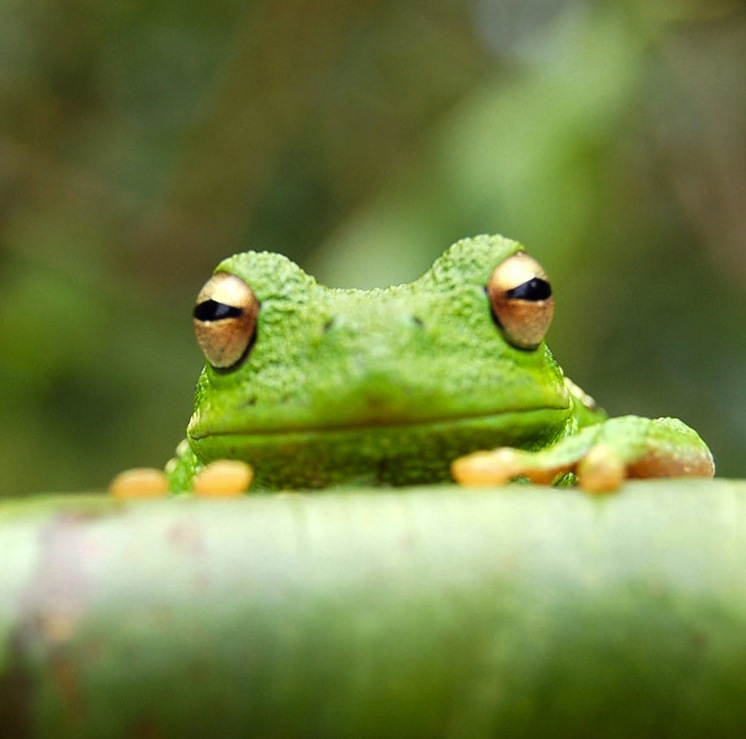
\includegraphics[width=0.5\textwidth]{figures/frog.jpg} 
	\caption{Βάτραχος}
	\label{frog_image}
\end{Illustration}
 
% % Βιβλιογραφία - Αναφορές
% 	\bibliography{references}
% % Συντομογραφίες - Αρκτικόλεξα - Ακρωνύμια
% 	\includeabbreviations{back_matter/abbreviations}
% % Γλωσσάριο
% 	\includeglossary{back_matter/glossary}
% %%%%%%%%%%%%%%%%%%%%%%%%%%%%%%%%%%%%%%%%%%%%%%%%%%%%
% % Ευρετήριο Όρων
% 	\printindices
%
%%%%%%%%%%%%%%%%%%
%%%%%%%%%%%%%%%%%%

%% Δημιουργία ετικετών CD:

	\definecdlabeloffsets{0}{-0.65}{0}{0.55} % upper label x offset [cm] (default=0) /  upper label y offset [cm] (default=0) /  lower label x offset [cm] (default=0) /  lower  label y offset [cm] (default=0) -- For Q-Connect KF01579 labels use the following offset values: {0}{-0.65}{0}{0.55}

	\createcdlabel{Πρότυπο Σύστημα Ομότιμων \\ Κόμβων Βασισμένο σε Σχήματα \en{RDF}}{Κωνσταντίνος Δ. Δημητρίου}{ΟΚΤΩΒΡΙΟΣ}{2020}{8} % τίτλος διπλωματικής / όνομα συγγραφέα / μήνας / έτος / εύρος περιοχής τίτλου σε cm (προτεινόμενη τιμή: 8) 

%%σ
%% Δημιουργία εξωφύλλου θήκης CD:

	\createcdcover{Πρότυπο Σύστημα Ομότιμων \\ Κόμβων Βασισμένο σε Σχήματα \en{RDF}}{Στάμος Φ. Ευάγγελος}{ΟΚΤΩΒΡΙΟΣ}{2020}{10} % τίτλος πτυχιακής / όνομα συγγραφέα / μήνας / έτος / εύρος περιοχής τίτλου σε cm (προτεινόμενη τιμή: 10) 

%%
%
\end{document}

%%%%%%%%%%%%%%%%%%%%%%%%%%%%%%%%%%%%%%%%%%%%%%%%%%%%
